\documentclass[preprint,12pt,authoryear]{elsarticle}

\usepackage{amsmath}
\usepackage{amssymb}
\usepackage{booktabs}
\usepackage{multirow}
\usepackage{natbib}
\usepackage{graphicx}

\journal{Energy Economics / Resources Policy (target journal to be confirmed)}

\begin{document}

\begin{frontmatter}

\title{Bayesian Latent Stochastic Volatility Models for Cocoa, Gold, and Crude Oil: A Comparative Risk Assessment for Ghana and West Africa}

\author{Jonathan}
\affiliation{organization={Independent Researcher},
            addressline={},
            city={},
            postcode={},
            state={},
            country={Ghana}}

\begin{abstract}
\noindent
Cocoa underpins the livelihoods of a large share of Ghanaian smallholder farmers, gold is one of the country's principal export and fiscal revenue sources, and crude oil is a major import exposure with direct fiscal and balance-of-payments consequences, yet no existing study we identified applies a rigorously backtested Bayesian latent stochastic volatility framework across all three commodities for a West African economic context. We estimate four Bayesian latent stochastic volatility specifications --- a Gaussian base model, and extensions incorporating Student-$t$ innovations, an exactly derived leverage channel, and their combination --- alongside four standard benchmarks (GARCH, EGARCH, Ornstein--Uhlenbeck, and Historical Simulation), and evaluate all eight against a pre-registered, rolling-window out-of-sample Value-at-Risk and Expected Shortfall backtesting framework comprising three complementary statistical tests. The results do not support a single dominant specification. Student-$t$ stochastic volatility models --- with and without an additional leverage channel --- achieve a perfect backtest pass rate for both gold and cocoa, with the leverage variant producing the smallest deviation from nominal coverage of any specification we estimate for cocoa specifically, consistent with a genuine, if modest, asymmetric volatility response particular to that commodity; and no model we estimate, including the richest specification available to us, adequately captures oil's 99\% Value-at-Risk. This differentiated outcome is itself the paper's central contribution: a commodity-specific account, established under an evaluation framework committed to in writing before any result was seen, of where Bayesian latent stochastic volatility earns its additional complexity for three commodities of direct relevance to a West African economy, and where, notably for oil, it does not.
\end{abstract}

\begin{highlights}
\item Bayesian stochastic volatility models are backtested for cocoa, gold, and oil.
\item SV-t achieves a perfect VaR/ES backtest pass rate for gold.
\item SV-t-Leverage is the only model to pass all backtests for cocoa.
\item No model tested adequately captures oil's 99\% Value-at-Risk.
\item Evaluation framework was pre-registered before any model was estimated.
\end{highlights}

\begin{keyword}
Bayesian stochastic volatility \sep Value-at-Risk \sep Expected Shortfall \sep commodity price risk \sep cocoa \sep gold \sep crude oil \sep Ghana \sep West Africa
\end{keyword}

\end{frontmatter}

\section{Introduction}
\label{sec:introduction}

A cocoa farmer in Ghana's Ashanti or Western Region does not experience a price movement on the ICE futures exchange as an abstract statistic. It arrives, months later and once removed through COCOBOD's producer-price mechanism, as the number that determines whether a season's harvest covers a household's costs. Gold, mined and exported in substantial volume, feeds directly into government revenue and the country's external accounts. Crude oil, imported rather than produced, does the reverse: a price spike raises the cost of fuel, transport, and electricity generation across the economy, with fiscal and balance-of-payments consequences that a finance ministry cannot simply absorb. These three commodities are not interchangeable entries on a list of things Ghana trades. Each carries a distinct kind of exposure, and this paper is built around the premise that a serious account of commodity price risk for this economy needs to take that distinction seriously rather than treat cocoa, gold, and oil as three instances of the same underlying problem.

\subsection{The Research Gap}

Bayesian latent stochastic volatility modelling is not a new or unproven methodology. Its foundations were established by \citet{jacquierpolsonrossi1994} and developed into the likelihood-based estimation framework we build on directly by \citet{kimshephardchib1998}, and the approach has since been applied across a wide range of financial markets. It has, moreover, already been applied to Ghanaian financial data specifically: \citet{tweneboah2025} estimate a family of Bayesian stochastic volatility models, including a leverage-effect specification, on the Ghana Stock Exchange Composite Index. That paper is the closest methodological precedent to our own, and we return to it directly in Section~\ref{sec:discussion}. But it is an application to a single domestic equity index, not to commodities, and not to the specific tail-risk backtesting question this paper asks.

A separate and genuinely valuable strand of literature examines how cocoa, gold, and oil prices relate to Ghana's broader macroeconomy: \citet{boateng2022} study the interconnectedness of cocoa, Brent crude, and gold with Ghana's real sector; \citet{yeboah2025} examine asymmetric dependence between these same commodities and Ghanaian macroeconomic variables including the exchange rate and inflation; and \citet{barson2023} use wavelet methods to study exchange-rate-conditioned commodity comovement. These studies ask an important and different question from ours: whether and how commodity prices move together with Ghana's exchange rate, inflation, and real economic activity. None of them asks whether a given commodity's own volatility can be adequately modelled and backtested in the first place, independent of any macroeconomic conditioning variable --- which is the question this paper takes up directly.

Putting these two strands together, the gap this paper addresses can be stated precisely rather than sweepingly: no study we identified in the course of preparing this paper applies a Bayesian latent stochastic volatility framework, evaluated against a genuine out-of-sample Value-at-Risk and Expected Shortfall backtesting exercise, across cocoa, gold, and crude oil specifically for a West African economic context. We make no claim that such a study does not exist anywhere; we report only that a careful search did not locate one, and that the combination of commodities, methodology, and evaluation rigour this paper brings together does not appear to have been assembled before.

\subsection{Why These Three Commodities Together}

Cocoa, gold, and oil are not grouped in this study as a matter of convenience. Each occupies a distinct position in Ghana's economy --- an agricultural export tied directly to rural livelihoods, a mined export tied to national fiscal revenue, and an energy import tied to the cost side of the economy rather than the revenue side --- and, as the data analysis in Section~\ref{sec:data} establishes in full, each poses a genuinely different statistical modelling challenge. Cocoa's return series shows a detectable asymmetric volatility response to negative shocks; gold's does not, or not strongly enough to matter; and oil's return distribution is shaped by a small number of episodes so extreme that standard measures of tail thickness place it in a different category altogether from either of the other two. A study that tested only one of these commodities could not have discovered that the right model differs so clearly by commodity. The comparative design is deliberate, not incidental, precisely because we did not know in advance whether one specification would suffice for all three, and we do not think a reader should be asked to take on faith that it would.

\subsection{Research Question}

The question this paper answers is direct: do Bayesian latent stochastic volatility models, and if so which specific variant, produce adequately calibrated Value-at-Risk and Expected Shortfall forecasts for cocoa, gold, and crude oil, relative to standard GARCH-family, mean-reverting, and non-parametric benchmarks, under a rolling out-of-sample backtesting framework specified and committed to in advance of estimation? And, following directly from the discussion above, is the answer to that question the same across all three commodities, or genuinely different?

We can say now, without pre-empting the results themselves, that the answer is the latter. The remainder of this paper is organised around establishing, commodity by commodity, exactly where a richer volatility specification earns its complexity and where even the richest specification we estimate does not.

\subsection{Contribution}

This paper's contribution is a commodity-differentiated, rigorously backtested comparison of Bayesian latent stochastic volatility against standard benchmarks for three commodities of direct relevance to Ghana and West Africa, using an evaluation framework --- window length, backtest statistics, and robustness checks alike --- fixed in writing before any model was estimated on real data. We do not claim to identify a single best model for commodity risk generally; we show, instead, precisely where a given specification's additional complexity is and is not justified, commodity by commodity, and we report this even where the answer, as it is for oil, is that none of the models we estimate clears the bar we set in advance.

\subsection{Roadmap}

Section~\ref{sec:literature} reviews the literature this paper builds on and departs from. Section~\ref{sec:data} describes the data underlying all subsequent analysis and establishes the stylised facts that motivate our model choices. Section~\ref{sec:methodology} sets out the full model specification, from the base stochastic volatility model through to the leverage and Student-$t$ extensions, together with the complete pre-registered evaluation framework. Section~\ref{sec:results} reports the results of that evaluation. Section~\ref{sec:discussion} discusses what those results mean in practice, situates them relative to the existing literature, and reports this study's limitations in full. Section~\ref{sec:conclusion} concludes.

\section{Literature Review}
\label{sec:literature}

This section situates the present study against four strands of literature: the foundations of Bayesian stochastic volatility estimation; the GARCH-family models we use as benchmarks; applications of stochastic volatility to commodity and energy markets specifically; and the Ghana-specific literature on commodity prices and the macroeconomy. We draw only on sources whose bibliographic details we have independently verified, and we say so explicitly where a detail remains unconfirmed rather than presenting an uncertain citation as settled.

\subsection{Foundations of Bayesian Stochastic Volatility}

The Bayesian estimation of latent stochastic volatility models originates with \citet{jacquierpolsonrossi1994}, who developed Markov Chain Monte Carlo methods for the basic discrete-time SV specification, treating log-volatility as an unobserved state rather than a deterministic function of past returns. \citet{kimshephardchib1998} extended this framework with a likelihood-based approach permitting direct comparison against ARCH-type models, and it is this specification, in its base Gaussian form, that we adopt as the starting point for our own SV-Gaussian model in Section~\ref{sec:sv}. \citet{jacquierpolsonrossi2004} subsequently extended the original framework to accommodate fat-tailed innovations and correlation between return and volatility shocks --- the two extensions, Student-$t$ innovations and leverage, that form the core of our own SV-$t$ and SV-Leverage specifications.

A specific computational problem in this literature bears directly on our own implementation. \citet{kastnerfruhwirthschnatter2014} showed that the choice between a centred and a non-centred parameterisation of the latent log-volatility path materially affects MCMC sampling efficiency, with the centred form performing poorly precisely in the high-persistence regime that characterises most financial and commodity return series. \citet{hosszejnikastner2019} extended this analysis specifically to the SV model with leverage, deriving both centred and non-centred samplers for the correlated case. We encountered exactly the identification and mixing difficulty this literature describes during our own initial implementation of the centred parameterisation, and our adoption of the non-centred form --- and the exact leverage derivation it makes possible, detailed in Section~\ref{sec:leverage} --- follows directly from this line of work.

\subsection{GARCH-Family Benchmarks}

Our benchmark specifications draw on two foundational contributions to the GARCH literature. \citet{bollerslev1986} introduced the GARCH(1,1) model itself, and \citet{nelson1991} introduced the exponential GARCH specification that allows an asymmetric volatility response to positive and negative shocks. Our decision to fix the order of both models at $(1,1)$ a priori, rather than search across orders on our own data, rests on \citet{hansenlunde2005}, whose systematic comparison of 330 ARCH-type specifications against exchange-rate data found that no higher-order model significantly outperformed GARCH(1,1) out-of-sample --- a finding we treat as a warrant for fixing this choice in advance rather than as license to skip a genuine robustness check, which we report separately in Section~\ref{sec:evaluation}.

\subsection{Stochastic Volatility and Commodity Markets}

The application of stochastic volatility methods to commodity and energy markets specifically provides the closest empirical precedents to our own work, and here the pattern in the literature is instructive rather than uniform. \citet{trolleschwartz2009} develop an affine commodity-derivatives pricing model incorporating unspanned stochastic volatility, providing a theoretical justification for treating commodity volatility as containing risk not fully captured by observable futures-curve movements --- a justification for the latent-volatility approach we adopt throughout this study, even though our own models are estimated directly on returns rather than through a derivatives-pricing lens.

Two studies applying Bayesian stochastic volatility directly to oil returns reach opposite conclusions about the value of heavy-tailed innovations, and we treat this contrast as substantively important rather than a minor inconsistency to note in passing. \citet{chenzerillibaum2019}, estimating Bayesian SV models with Gaussian, Student-$t$, and asymmetric Laplace innovations on spot oil returns using a pre-2018 sample, find that the Gaussian specification performs best out-of-sample for their Value-at-Risk and Conditional Value-at-Risk applications. \citet{kuang2022}, whose sample spans the 2008 financial crisis through the COVID-19 pandemic, reaches the opposite conclusion: flexible distributions capturing both skewness and fat tails are necessary for adequate oil tail-risk forecasting over that window. We return to this contrast directly in our own discussion of the oil results in Section~\ref{sec:results_oil} and Section~\ref{sec:discussion}, since our own finding --- that no model we estimate, including Student-$t$ and leverage extensions, adequately captures oil's 99\% VaR over a sample that includes both the COVID-19 period and the 2026 Middle East conflict --- sits naturally alongside \citet{kuang2022}'s result rather than \citet{chenzerillibaum2019}'s.

Agricultural commodity volatility has received comparatively less attention within the Bayesian SV literature specifically, though the broader GARCH-family literature offers a directly relevant precedent for our own cocoa result. \citet{roux2018} compare GARCH, GJR-GARCH, and EGARCH specifications across cocoa, coffee, sugar, and several financial series, and find that only cocoa, among the commodities studied, shows a leverage effect detectable through the GJR-GARCH asymmetry term. This is an independent, differently modelled confirmation of the pattern our own results establish for cocoa specifically in Section~\ref{sec:results_cocoa}.

Finally, on the choice of benchmark for mean-reversion in commodity price levels, \citet{bessembinderetal1995} provide the classical evidence underlying our expectations for the Ornstein--Uhlenbeck specification: their analysis of futures term structures finds economically large mean reversion for agricultural commodities and crude oil, but substantially weaker reversion for precious metals. As reported in Section~\ref{sec:results_ou}, our own OU non-convergence diagnostic --- built for an unrelated purpose, to flag windows where mean-reversion could not be reliably estimated --- reproduces this thirty-year-old pattern directly, with gold showing more than double the non-convergence rate of either cocoa or oil.

\subsection{Ghana and West African Commodity-Macroeconomy Literature}

A distinct body of work examines the relationship between commodity prices and Ghana's broader macroeconomy, and we position our own study carefully alongside it rather than as an extension of it. \citet{boateng2022} study the interconnectedness of cocoa, Brent crude oil, and gold with Ghana's real sector, establishing that these three commodities are not merely traded internationally but measurably connected to domestic economic activity. \citet{yeboah2025} examine asymmetric dependence between cocoa, crude oil, gold, and Ghanaian macroeconomic variables including the exchange rate and inflation using a quantile-on-quantile approach, reporting nonlinear and asymmetric relationships across the variables studied. \citet{barson2023} use wavelet coherence methods to study comovement between Ghanaian commodity returns and exchange rates across different time horizons.

These three studies ask a genuinely different question from the one this paper answers. They examine dependence and comovement between commodity prices and macroeconomic variables; we examine whether a given commodity's own return volatility can be adequately modelled and backtested at all, independent of any macroeconomic conditioning variable. The two research questions are complementary rather than competing, and we note, as a direction for future work in Section~\ref{sec:discussion}, that conditioning the volatility models estimated in this paper on the exchange-rate and macroeconomic variables this literature has already shown to matter is a natural extension we have not attempted here.

The single closest methodological precedent to our own work is \citet{tweneboah2025}, who apply Bayesian stochastic volatility models --- including linear-regressor, Student-$t$, leverage, and combined Student-$t$-with-leverage variants --- to the Ghana Stock Exchange Composite Index over 2011--2022, identifying the Student-$t$ specification as most effective by root-mean-squared error.\footnote{We have confirmed the substance of this study directly but have not independently confirmed the exact volume and issue number of its publication in \textit{Risks} (MDPI), and we flag this rather than present an unconfirmed detail as settled.} This is, to our knowledge, the only prior application of this exact model family to Ghanaian financial data, and it applies to a domestic equity index rather than to internationally traded commodities. Our own study extends this methodological approach to cocoa, gold, and crude oil specifically, and evaluates it against a pre-registered out-of-sample VaR and Expected Shortfall backtesting framework rather than in-sample fit criteria alone.

\subsection{Positioning This Study}

Taken together, this literature establishes that Bayesian latent stochastic volatility is a mature and well-validated methodology, that its extensions to fat tails and leverage are well understood in general and have identifiable computational pitfalls we ourselves encountered and resolved, that its application to commodity markets specifically produces genuinely different conclusions depending on which crises a given sample happens to include, and that it has been applied once to Ghanaian financial data, though not yet to commodities. No study we identified brings a rigorously backtested version of this methodology to cocoa, gold, and crude oil together for a West African economic context, which is precisely the gap this paper addresses.

\section{Data}
\label{sec:data}

Every empirical claim in this paper rests on three daily price series
— cocoa, gold, and Brent crude oil — and on a set of decisions about
how those series were assembled, validated, and cleaned before a
single volatility model touched them. We describe that process in
full here, including the parts that did not resolve neatly, because a
risk model is only as trustworthy as the price series feeding it, and
because commodity data of the kind used in this study is messier than
it first appears.

\subsection{Sources and Provenance}
\label{sec:sources}

\subsubsection{Cocoa}

Cocoa prices are the daily closing price of the ICE cocoa continuous
front-month futures contract, ticker CC=F, retrieved from Yahoo
Finance in USD per tonne. This is a retail-accessible series, not an
exchange-licensed feed, and we want to be upfront about what that
means: Yahoo does not publish the roll methodology by which its
continuous series is stitched together from successive individual
contracts, and no free source we could locate does either for cocoa
specifically. Institutional data vendors such as Bloomberg or
Refinitiv document this precisely; a solo researcher without
institutional access does not have that option, and we treat the
consequence of that constraint as a stated limitation rather than
something to paper over.

To have any independent check on this series at all, we cross-validated
it against the official daily reference price published by the
International Cocoa Organization (ICCO), which is itself constructed
as an average of London and New York futures quotations converted to
US dollars at prevailing exchange rates. Across the full window for
which we could obtain both series (essentially the entire 2000--2025
period, using an official ICCO export supplemented by a third-party
archival source described below), the two series correlate at 0.99 —
strong enough to conclude they track the same underlying market — but
diverge in level by a mean of 3.8\%, with individual days reaching
20\% or more. That is a substantial gap for two series purporting to
measure the same thing, and it does not resolve into either series
simply being wrong. ICCO's own published methodology states that its
composite price averages the nearest three active contract months,
not the front month alone; Yahoo's CC=F, by contrast, is a single-contract
continuous series. Restricting the comparison to ICCO's New York leg
in isolation — still a blend of nearby months, but a narrower one —
reduces the mean discrepancy to 2.0\%, which confirms that
contract-month averaging accounts for roughly half the gap. It does
not account for the other half. We tested and ruled out a simple
timing lag (shifting either series by one trading day made the fit
worse, not better), and we are not able to offer a confirmed
explanation for the residual 2\% beyond that point. We report this as
an open item rather than force a tidy resolution onto it.

A second complication concerns the pre-2024 portion of the ICCO
series. ICCO's own free access to historical daily prices stops at
2024; earlier data sits behind a paid product. We located a
third-party repository on Kaggle (uploader: achazngwouanzi) claiming
to reproduce ICCO's daily prices from 1994 onward, citing ICCO as the
original data owner. Before using any part of this file, we checked
it against our independently obtained, official ICCO export for the
window where both existed: 219 overlapping trading days from October
2024 to August 2025. Every single value matched to the cent — zero
discrepancy across all 219 observations. That is a real, strong
validation for the window we could check, and it is the basis on
which we extended our cocoa cross-validation back to 1994 using the
Kaggle file. It is not, strictly, a validation of the pre-2024 portion
itself, since we have no independent ground truth for those years; we
are relying on the reasonable inference that a file which reproduces
recent ICCO data exactly is likely — though not provably — to have
handled the earlier years with the same fidelity.

\subsubsection{Gold}

Gold prices are the daily closing price of the COMEX gold continuous
front-month futures contract, ticker GC=F, again from Yahoo Finance,
denominated in USD per troy ounce. The natural benchmark for
cross-validating a gold price series is the LBMA (London Bullion
Market Association) daily fixing, historically distributed through
the Federal Reserve's FRED database. That series, however, was
permanently removed from FRED at the end of January 2022, following
the announcement that FRED would no longer carry data from the ICE
Benchmark Administration, and it is not otherwise freely available in
bulk; the World Gold Council removed the equivalent historical series
from its own site in 2025 pending a licensing arrangement. We
mention this in some detail because it changes the honest baseline
for what validation is achievable for gold specifically: not every
commodity in this study had an equally good free alternative
available, and gold's validation had to be built around a different
source than we would have preferred.

That alternative was Stooq, a commercial market-data aggregator whose
free daily XAU/USD series we downloaded directly. Before trusting it,
we inspected the raw file and found something worth flagging on its
own: rows before 1970 were not genuine daily observations at all.
They repeated the same price four times a year in a quarterly pattern
— for instance, the 1793 entries showed an identical value of 19.39
on four separate dates spaced roughly a quarter apart — which is the
signature of a flat-filled placeholder standing in for data the
provider did not actually have, not a real market price. We excluded
this entire pre-1970 portion and restricted the cross-validation to
the genuinely daily-frequency section of the file, 1970 onward.
Within that restricted window, agreement with our Yahoo Finance GC=F
series was strong: across 6{,}457 overlapping trading days spanning
2000 to 2026, the two series correlate at 1.00 and differ by a mean
absolute 0.23\%, the tightest agreement of any cross-validation
exercise in this study. Stooq is not an audited, institutional
benchmark, and we do not claim it is one; what this comparison
establishes is that two independently sourced series are tracking the
same real market closely enough to give confidence in the gold price
data used here, which is the practical question that matters for a
risk model.

\subsubsection{Oil}

The choice of oil benchmark deserves more explanation than the other
two commodities, because it is not simply a matter of which free
source was easiest to obtain. The commodity finance literature and
retail data providers alike default to West Texas Intermediate (WTI),
the US benchmark. We use Brent instead — specifically, the daily
Brent-Europe spot price published by the US Energy Information
Administration and distributed through FRED as series DCOILBRENTEU —
as our primary oil series, and we want to explain why this is not a
cosmetic substitution.

Brent is the internationally relevant reference price for oil traded
into and out of West Africa; Ghana's own oil exports and regional
pricing conventions reference Brent, not WTI. That alone would be
reason enough to prefer it for a paper framed around West African
commodity risk. But there is a sharper, empirical reason as well. On
April 20, 2020, the expiring May 2020 WTI futures contract settled at
$-\$37.63$ per barrel, and the following day's contract closed at
$+\$10.01$, as storage capacity at the Cushing, Oklahoma delivery
point was exhausted by the collapse in demand triggered by COVID-19
lockdowns. We confirmed this directly in our own downloaded WTI
series (Yahoo Finance CL=F) rather than taking it on faith from
secondary reporting. Over the identical trading days, Brent spot did
not go negative at all; its low for that week was \$9.12. Two series
that are supposedly measuring "the price of oil" behaved in
qualitatively different ways during the single most extreme episode
in either series' recent history. That is not a minor technical
distinction. It is direct evidence that Brent and WTI are separate
risk processes with separate contract mechanics, not interchangeable
proxies for a single underlying quantity, and it justifies treating
the choice between them as a substantive modelling decision rather
than an arbitrary one.

Having made that choice, we retained the WTI futures series as a
secondary, robustness-only series and cross-validated it against
FRED's own WTI spot series (DCOILWTICO, the spot price at Cushing).
Over 1{,}248 overlapping trading days from mid-2021 to mid-2026, the
Yahoo WTI futures series and the FRED WTI spot series correlate at
0.998 in price levels and 0.994 in log returns — a tight fit overall
— but with a basis (the gap between futures and spot) that is not
constant. It widens noticeably in 2024, a year in which WTI futures
are independently documented to have traded in backwardation for
roughly nine months before shifting toward contango in November, and
it widens again far more sharply in 2026, coinciding with a documented
spike in WTI to over \$119 per barrel in March 2026 following the
outbreak of conflict between the United States, Israel, and Iran in
late February, and the resulting disruption to Middle Eastern oil
flows. Both of those episodes give a real, dateable market-structure
explanation for the observed basis movements. What we cannot fully
explain is why the basis remained elevated through 2025 specifically,
a year for which the documented forecast at the time was a shift
toward full contango — the opposite of what a persistently wide,
futures-below-spot gap would suggest. We tested the obvious
alternative explanation, a simple reporting lag between the two
series, and found it did not improve the fit. We report this,
consistent with our general approach in this section, as an
unresolved discrepancy rather than a resolved one.

As a final check specific to Brent, we examined every daily return
exceeding five standard deviations from the mean across the full
sample — 47 such observations — and confirmed that essentially all of
them fall on dates independently associated with well-documented
historical events: the 1990 Iraqi invasion of Kuwait and the ensuing
Gulf War, the 1998 Asian financial crisis, the September 2001 attacks,
the 2008 global financial crisis, the March–May 2020 COVID collapse,
and the February–March 2026 Middle East conflict. We read this
pattern as evidence of data integrity rather than data error: a
volatility model built on this series is not being asked to explain
noise, but to explain a documented sequence of real market shocks.

\begin{table}[htbp]
\centering
\caption{Primary Data Sources and Cross-Validation Summary}
\label{tab:sources}
\small
\begin{tabular}{lllrr}
\toprule
Commodity & Primary series & Validation series & Correlation & Mean abs.\ diff. \\
\midrule
Cocoa & CC=F (Yahoo) & ICCO composite & 0.99 & 3.8\% \\
Gold  & GC=F (Yahoo) & Stooq XAU/USD (1970+) & 1.00 & 0.23\% \\
Oil (robustness) & CL=F (Yahoo, WTI) & FRED DCOILWTICO & 0.998 (levels) & 0.77\% \\
\bottomrule
\end{tabular}
\end{table}

\subsection{Common Sample Period}
\label{sec:sample}

All three models are estimated over the same window: January 1, 2003
to June 22, 2026. Two considerations fixed this choice. The gold
series is unavailable before August 30, 2000, which sets an absolute
floor on how far back any common sample can begin. More decisively,
both the cocoa and gold series show data-quality problems concentrated
disproportionately in their earliest years — the zero-volume issue in
cocoa and gold discussed in the next section is far more frequent
before roughly 2007 than after — and a 2003 start substantially, if
not completely, reduces exposure to that period without discarding
the majority of usable history. Within this common window, after all
cleaning steps described below, the modelling sample comprises 5{,}123
observations for cocoa, 5{,}893 for gold, and 5{,}806 for oil. The
differences across commodities reflect different holiday and
non-trading-day calendars across the three underlying exchanges, plus
the cleaning exclusions specific to cocoa and oil described
immediately below.

\subsection{Data Cleaning}
\label{sec:cleaning}

We commit, throughout this study, to a single governing principle:
no missing observation is filled in, and no observation is excluded
without a stated, diagnosable reason tied to a specific problem in
how that observation was recorded. This matters more here than it
might for many empirical exercises, because the object of study is
volatility itself. A forward-filled or interpolated price
mechanically understates the return, and hence the volatility, of
exactly the days on which the true volatility is least certain — which
is precisely backwards for a study whose purpose is to model tail
risk. We would rather report a shorter, honestly-gappy series than a
longer, artificially smoothed one.

\subsubsection{Cocoa: Zero-Volume Days}

Across the full raw cocoa series, 7.9\% of trading days show zero
recorded trading volume, and the frequency of these days increases
markedly in 2024 and 2025 relative to the middle years of the sample.
A day with zero volume typically also shows identical open, high, low,
and close prices — a strong indication that the "price" recorded for
that day is a stale settlement carried forward from the previous
session, not a genuine market-clearing observation, since a contract
with real trading activity does not typically print a perfectly flat
OHLC bar.

We wanted to know whether these days were a benign reporting artifact
or a genuine signal of something happening in the market — specifically,
whether they marked periods of contract-rollover illiquidity that
would corrupt the return series if left untreated. We tested this
directly rather than assuming an answer: for each zero-volume day, we
checked whether the following trading day showed an abnormally large
price move, on the logic that a rollover-driven illiquidity episode
should be followed by a volume surge and a price correction once
trading resumes. For cocoa, the specific pattern we found around three
dates in 2024 — May 13, May 16, and September 16 — was a run of
several consecutive near-zero-volume days immediately followed by a
sharp jump in volume and a large price move (in the range of 17\% to
23\%). This is close to a textbook rollover signature. It is also,
however, a period independently documented as one of extraordinary
genuine volatility in the cocoa market: prices reached a record
\$11{,}530 per tonne in June 2024 amid severe West African supply
shocks, and the broader 2024 crisis continued into the second half of
the year. We cannot fully separate the rollover-illiquidity
explanation from the genuine-volatility explanation using price data
alone, and we do not think it is honest to pretend we can. Our
resolution is procedural rather than interpretive: we treat these
zero-volume days as missing prior to return calculation throughout the
main analysis, and we report, as a stated robustness check in
Section~\ref{sec:robustness_status}, how the core cocoa findings change when the three
flagged dates are instead retained. This lets the reader judge how
much the result depends on a decision we were genuinely unable to make
with full confidence.

We ran the identical zero-volume diagnostic on gold, where 6.5\% of
days show zero volume, heavily concentrated in 2000--2007 rather than
growing over time as in cocoa. The result there was different and, we
think, informative by contrast: zero-volume days in gold were
\emph{less} likely to be followed by a large price move than a
randomly chosen day (3.1\% versus a 6.9\% base rate), which is the
opposite of what a rollover-illiquidity signature would predict. We
read this as evidence that gold's zero-volume days are an artifact of
sparser electronic reporting in the early years of this particular
data feed, not a market-structure problem, and we apply no exclusion
to gold on this basis.

\subsubsection{Oil: Negative and Undefined Prices}

As described above, the WTI futures series recorded a negative
settlement on April 20, 2020, and a near-zero settlement the following
day. A log return is undefined when the price is zero or negative, so
these two days cannot be silently included in any log-return
calculation without either crashing the computation or, worse, being
coerced into a spurious numerical value. We exclude both dates
explicitly wherever the WTI series is used. Because our primary oil
series is Brent, which did not exhibit this problem, the exclusion has
no bearing on the main results; it applies only to the WTI robustness
comparisons.

\subsection{Stylised Facts}
\label{sec:stylised}

Before specifying any model, we characterised the statistical
properties of all three log-return series
($r_{i,t} = \ln(P_{i,t}/P_{i,t-1})$) directly, both because doing so
is standard practice and because, in this case, the results
genuinely shaped which model features we judged necessary rather than
optional. Table~\ref{tab:stylised} reports the full set of statistics;
we discuss what each one rules in or out below.

\begin{table}[htbp]
\centering
\caption{Stylised Facts: Daily Log-Returns, 2003--2026}
\label{tab:stylised}
\small
\begin{tabular}{lrrr}
\toprule
& Cocoa & Gold & Oil (Brent) \\
\midrule
Observations & 5{,}123 & 5{,}893 & 5{,}806 \\
Mean (daily, \%) & 0.0056 & 0.0423 & 0.0124 \\
Annualised volatility (\%) & 34.26 & 18.22 & 41.75 \\
Minimum return (\%) & $-26.06$ & $-12.07$ & $-64.37$ \\
Maximum return (\%) & 12.80 & 8.64 & 41.20 \\
Skewness & $-0.660$ & $-0.541$ & $-2.122$ \\
Excess kurtosis & 8.549 & 6.626 & 82.559 \\
Jarque--Bera statistic & 15{,}937.8 & 11{,}044.4 & 1{,}650{,}371.9 \\
\quad $p$-value & $<0.001$ & $<0.001$ & $<0.001$ \\
Hill tail index $\hat{\alpha}$ ($k=100$) & 4.203 & 3.639 & 2.802 \\
ARCH-LM statistic (10 lags) & 178.716 & 312.345 & 1{,}208.578 \\
\quad $p$-value & $<0.001$ & $<0.001$ & $<0.001$ \\
ADF statistic & $-20.512$ & $-30.657$ & $-16.111$ \\
\quad $p$-value & $<0.001$ & $<0.001$ & $<0.001$ \\
$\mathrm{corr}(r_t, r^2_{t+1})$ & $-0.023$ & $-0.031$ & $-0.158$ \\
\bottomrule
\end{tabular}
\end{table}

\textbf{Non-normality.} The Jarque--Bera test rejects the null of
normality for all three series at $p < 0.001$, and the excess kurtosis
figures make clear why: even the least extreme of the three, gold at
6.6, is far beyond what a Gaussian distribution would produce. The
Hill tail index estimates place all three in the region conventionally
associated with heavy-tailed financial data ($2 < \hat{\alpha} < 5$),
with oil ($\hat{\alpha} = 2.80$) the heaviest and cocoa
($\hat{\alpha} = 4.20$) the least extreme of the three, though still
clearly non-Gaussian. This is the direct empirical motivation for
including Student-$t$, rather than exclusively Gaussian, innovations
in the primary stochastic volatility specification: a model that
assumes normal shocks will systematically underestimate the
probability of the kind of extreme move these series actually produce.

\textbf{Oil's kurtosis specifically} is large enough that it merits
its own discussion rather than a line in a table. An excess kurtosis
of 82.6 is not a modest departure from normality; it implies a return
distribution dominated, in a statistical sense, by a small number of
extraordinary observations. We do not think this is an artifact of
data error — the large-move dates driving it correspond to
independently confirmed historical crises, and the April 2020 episode
in particular reflects a genuine, well-documented physical constraint
(the exhaustion of storage capacity) rather than a modelling or
data-collection failure. It is, instead, a real feature of the series
that raises a genuine question about the limits of parametric
volatility modelling for this specific commodity: even a Student-$t$
innovation distribution, however heavy-tailed, is a single smooth
family of curves being asked to represent a return distribution shaped
substantially by a handful of qualitatively distinct crisis regimes.
Whether that is achievable, and how well, is an empirical question we
return to directly in the results, rather than one we resolve here by
assumption.

\textbf{Volatility clustering.} Engle's ARCH-LM test rejects the null
of no ARCH effects for all three series at $p < 0.001$, confirming
that periods of high and low volatility cluster in time rather than
volatility being constant. This is the basic empirical fact that rules
out the constant-volatility Ornstein--Uhlenbeck specification as an
adequate description of any of the three series on its own terms,
independent of how it performs in the formal backtests reported later;
the data itself says volatility moves over time, so a model that
assumes it does not is misspecified from the outset for these
purposes, whatever else it might be useful for.

\textbf{Stationarity.} The Augmented Dickey--Fuller test rejects the
null of a unit root for all three log-return series at $p < 0.001$,
which is expected — log-returns of a price series are conventionally
stationary even when the price level itself is not — but is worth
confirming directly rather than assuming, since every model estimated
in this paper treats the return series as its stationary input.

\textbf{Asymmetric volatility response.} The correlation between
today's return and tomorrow's squared return is negative for all
three commodities, which is consistent with — though not on its own
proof of — a leverage effect, whereby a negative price shock raises
subsequent volatility by more than a positive shock of equal size
raises it. The magnitude differs meaningfully across commodities:
oil's correlation of $-0.158$ is substantial and, we think,
economically sensible, since a sharp oil price decline is often tied
to demand-side shocks (recession fears, or in 2020, an actual collapse
in physical demand) that carry genuine forward-looking uncertainty.
Cocoa and gold, at $-0.023$ and $-0.031$ respectively, show only a
mild version of the same pattern --- present, but weak enough that we
do not treat it as confirmed without a formal test. We build this
distinction into the model specification directly, by estimating both
leverage and non-leverage variants for every commodity and letting the
backtest evidence, not this preliminary correlation, determine which
specification the data actually supports.

\begin{figure}[htbp]
\centering
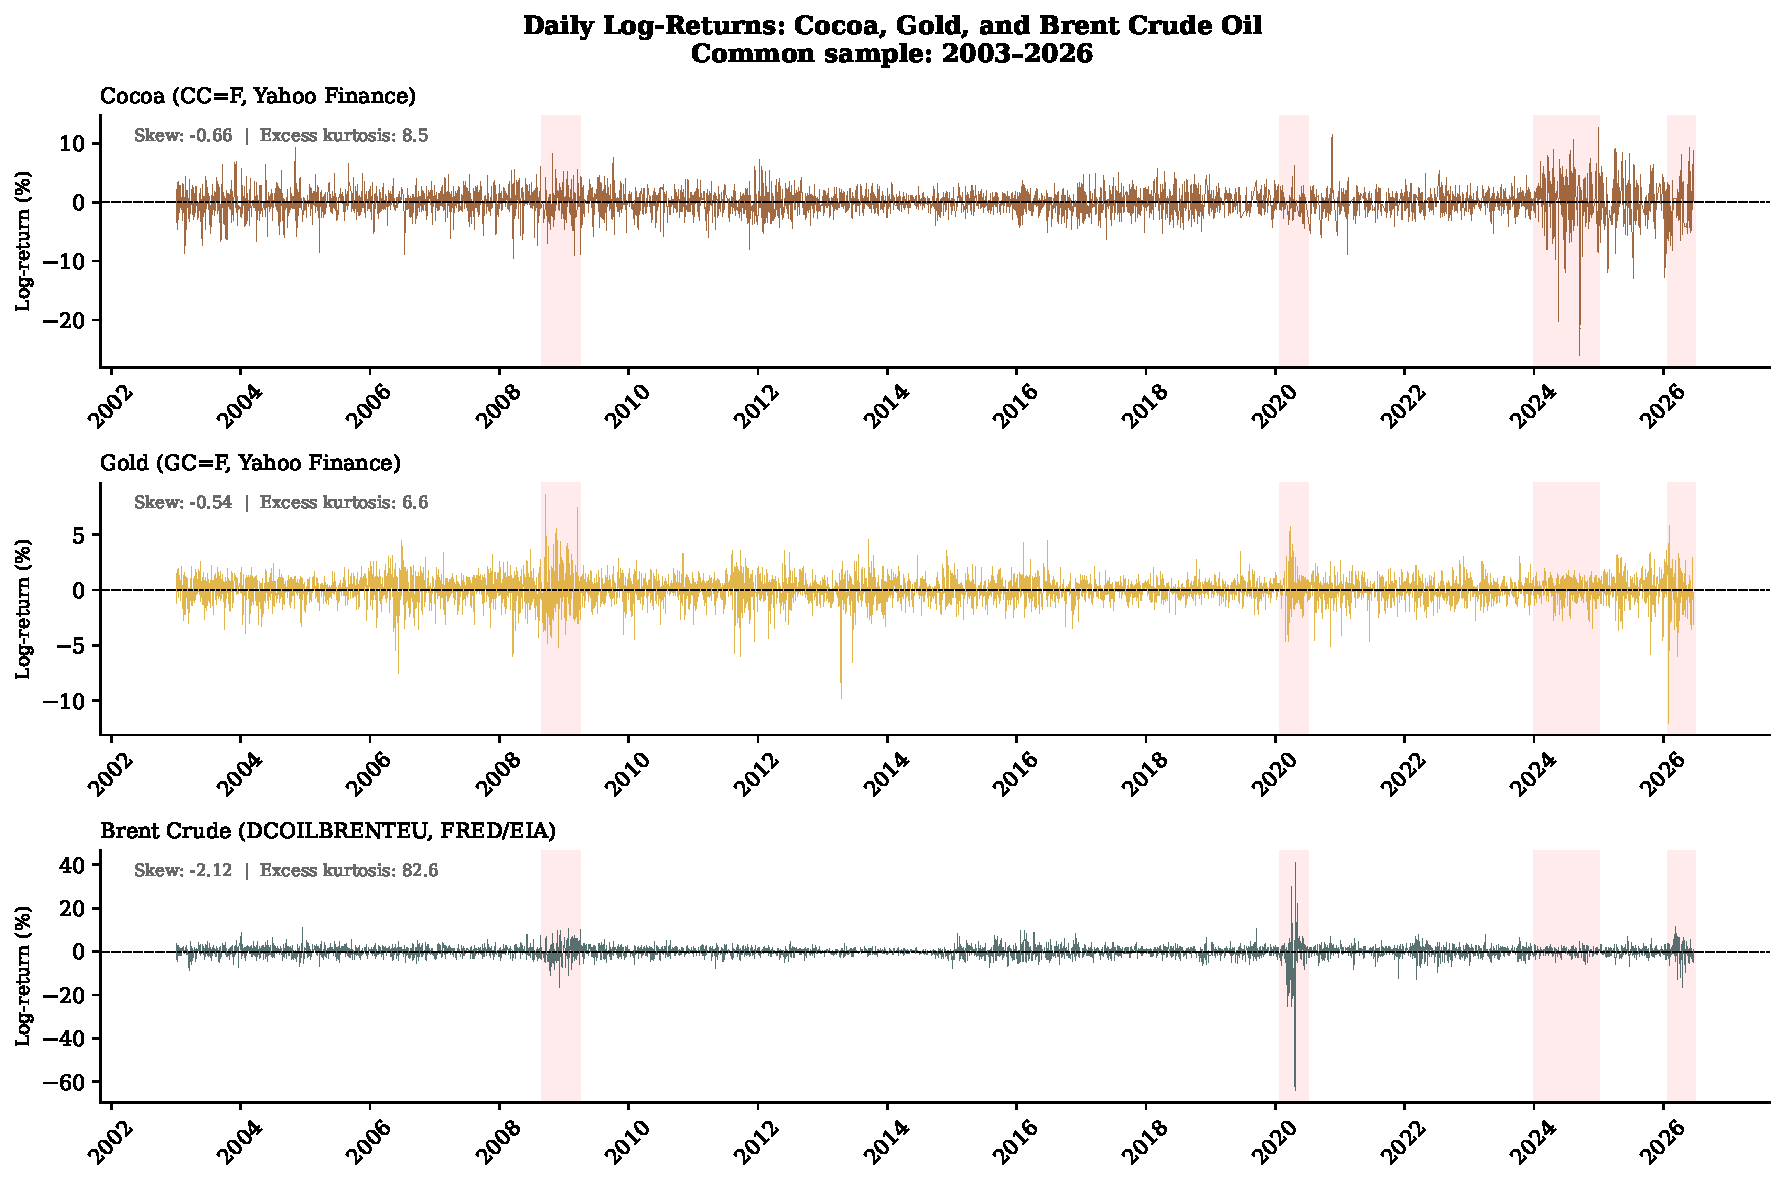
\includegraphics[width=\textwidth]{figs/fig1_returns_overview.pdf}
\caption{Daily log-returns for cocoa, gold, and Brent crude oil, 2003--2026. Shaded bands mark the four crisis episodes discussed throughout this paper: the 2008 global financial crisis, the 2020 COVID-19 collapse, the 2024 cocoa price crisis, and the 2026 Middle East-driven oil disruption. Oil's return scale is visibly wider than the other two series, consistent with the excess kurtosis reported in Table~\ref{tab:stylised}.}
\label{fig:returns_overview}
\end{figure}

\begin{figure}[htbp]
\centering
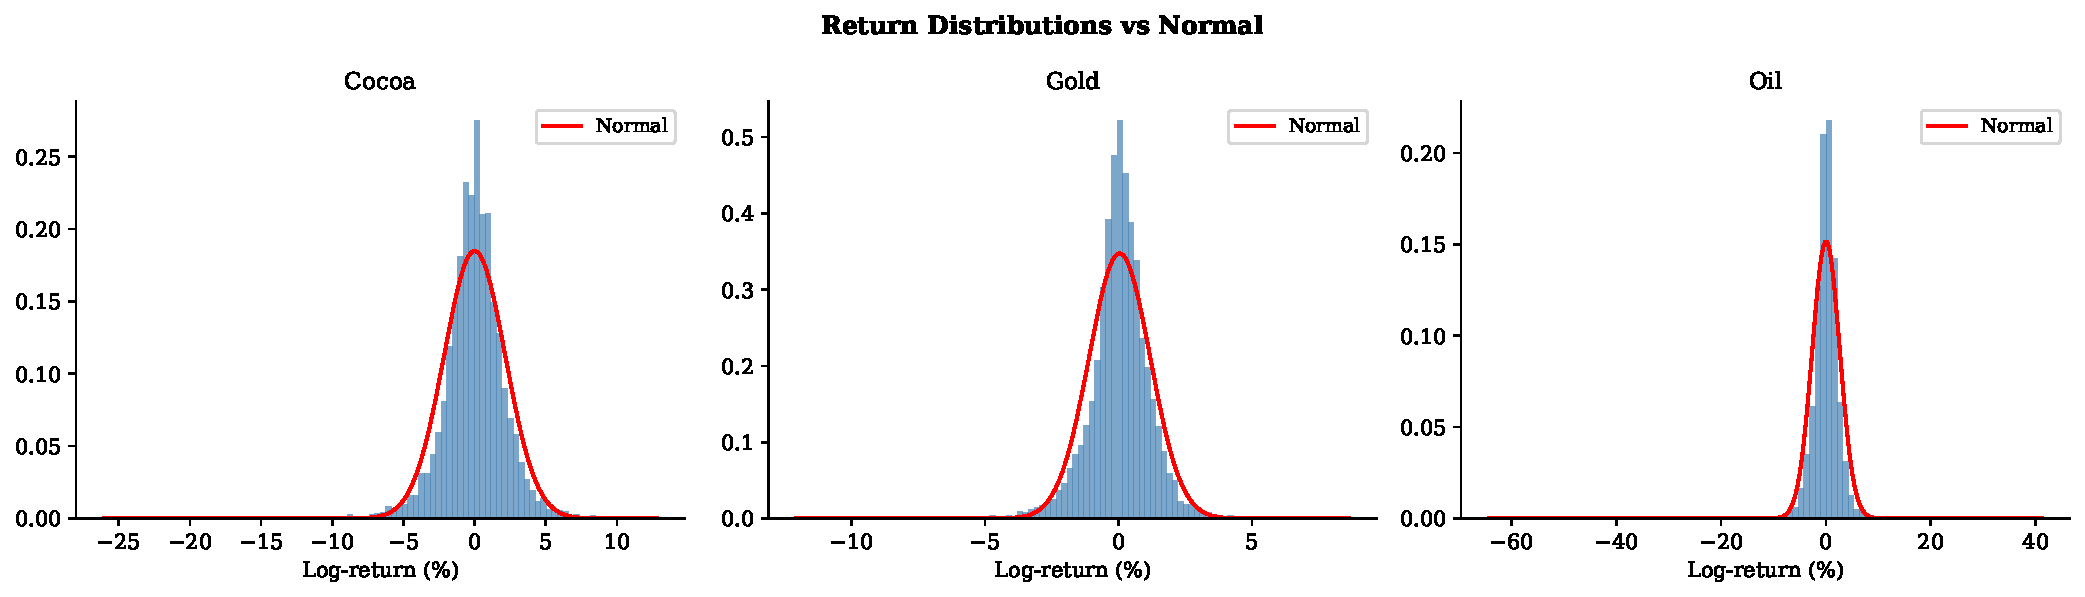
\includegraphics[width=\textwidth]{figs/fig2_distributions.pdf}
\caption{Empirical return distributions against a fitted normal density with matching mean and variance, for all three commodities. All three series show visibly heavier tails and a sharper central peak than the normal curve; this departure is most extreme for oil, consistent with the Jarque--Bera and Hill tail-index results reported in Table~\ref{tab:stylised}.}
\label{fig:distributions}
\end{figure}

\begin{figure}[htbp]
\centering
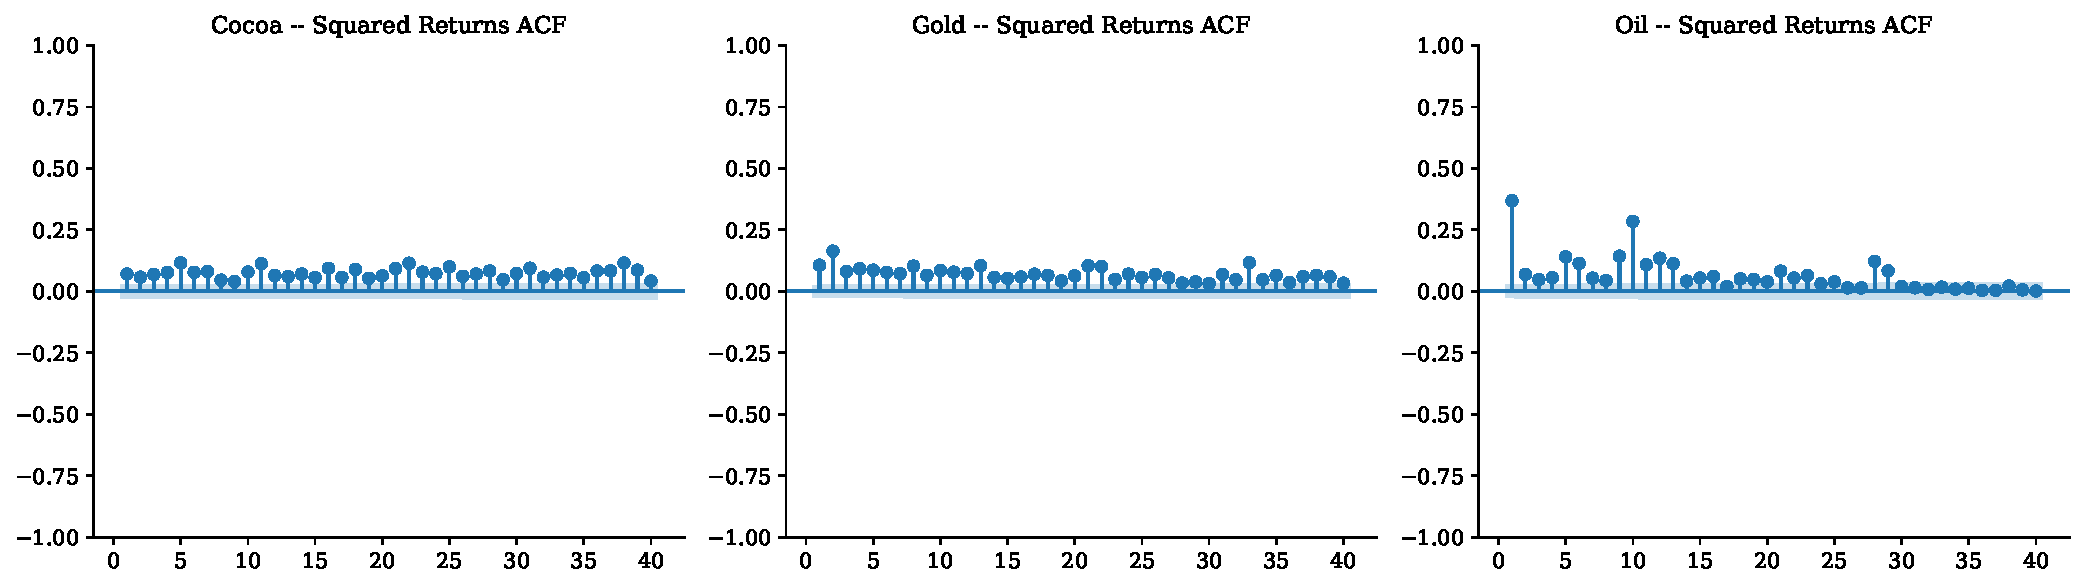
\includegraphics[width=\textwidth]{figs/fig3_acf_squared.pdf}
\caption{Autocorrelation function of squared daily returns, 40 lags, for cocoa, gold, and Brent crude oil. Persistent, statistically significant positive autocorrelation confirms volatility clustering for all three series and directly motivates the GARCH-family and stochastic-volatility specifications developed in Section~\ref{sec:methodology} over the constant-volatility Ornstein--Uhlenbeck benchmark.}
\label{fig:acf}
\end{figure}

\subsection{Ethics and Data Governance}
\label{sec:ethics}

This study uses exclusively public, freely available commodity price
data. It involves no human subjects, no personally identifiable
information, and no animal or clinical research of any kind, and
accordingly required and received no institutional ethics review. We
state this plainly rather than leave it implicit, since the absence of
an ethics review is itself a substantive fact about the study's scope
that some readers will reasonably want confirmed rather than assumed.

Where we relied on a source that is not the original data owner —
specifically, the Kaggle-hosted extension of ICCO's cocoa price series
— we have tried to be explicit about that distinction throughout: ICCO
is credited as the data's origin, the third-party route is disclosed,
and the validation exercise we performed against an independently
obtained official export is reported in full rather than glossed as
an afterthought. We think this level of disclosure matters more, not
less, for a solo researcher without institutional data infrastructure,
because the alternative — treating a convenient secondary source as
equivalent to a licensed institutional feed without saying so — is
precisely the kind of quiet shortcut that erodes trust in independent
empirical work.

There is a further point worth making, one that goes beyond formal
compliance. Cocoa is not, for Ghana, an abstract financial instrument.
It is the crop that a large share of Ghanaian smallholder farmers
depend on directly for their livelihoods, and the price volatility
this paper models has real consequences for household income, for
COCOBOD's hedging decisions, and for the country's export earnings, in
a way that gold and oil volatility, while economically significant in
their own right, do not carry in quite the same immediate, personal
sense for the researcher writing this. We do not think a technical
risk-modelling paper needs to moralise about this, and we have tried
not to. But we also do not think it is honest to model cocoa exactly
as if it were interchangeable with gold or oil purely because the
mathematics is the same, without acknowledging that the people on the
other end of this price series have no voice in how international
futures markets set the number this paper is trying to forecast. We
return to this point briefly in the discussion, where we consider what
the practical implications of our results might be for risk management
at the level of an institution like COCOBOD, rather than only for an
academic audience.

Finally, as with quantitative risk research generally, the methods
developed here could in principle be used by market participants whose
interests are not aligned with producer welfare — a more accurate
volatility forecast is, after all, a tool that can be used for hedging
or for speculation with equal technical validity. We regard this as a
standard, non-unique feature of financial risk modelling rather than a
reason to withhold methodological detail, but we note it rather than
pretend the distinction between these two uses is not real.

\subsection{From Data to Model}

What this data analysis establishes, taken together, is a clear and
specific modelling problem rather than a vague one. All three series
are volatile in a time-varying, clustered way that a constant-volatility
model cannot capture; all three depart from normality strongly enough
that Gaussian innovations are an inadequate assumption; cocoa and, more
substantially, oil show evidence of asymmetric volatility response to
negative shocks; and oil's return distribution is shaped by tail events
extreme enough to raise a genuine question about whether any standard
parametric specification can fully accommodate it. The remainder of
this paper is, in a real sense, an attempt to find out how far a
carefully specified Bayesian stochastic volatility model can go in
addressing exactly these four features, commodity by commodity, and
where --- as the results in Section~\ref{sec:results_oil} show plainly for oil --- it
cannot.
\section{Methodology}
\label{sec:methodology}

This section sets out, in full and in advance of any result, every model we estimate, every prior we place, and every criterion by which we judge one specification better than another. We take this ordering seriously. Everything described in Section~\ref{sec:evaluation} below was fixed before a single model was fitted to the data described in Section~\ref{sec:data}, and we return to this point explicitly because it is what separates a genuine backtesting exercise from a comparison quietly reverse-engineered from results already in hand.

\subsection{Notation}

Let $P_{i,t}$ denote the closing price of commodity $i \in \{\text{cocoa}, \text{gold}, \text{oil}\}$ on trading day $t$, and let
\begin{equation}
  r_{i,t} = \ln\!\left(\frac{P_{i,t}}{P_{i,t-1}}\right)
  \label{eq:logreturn}
\end{equation}
denote the corresponding daily log-return. Every model below is estimated separately for each commodity; nothing in this study models cocoa, gold, and oil jointly, since the research question concerns within-commodity model adequacy rather than cross-commodity dependence.\footnote{We return to this scoping decision explicitly in Section~\ref{sec:outofscope}.} One data-specific exception to Equation~\ref{eq:logreturn} arises for the WTI robustness series discussed in Section~\ref{sec:data}: the return is undefined on the two trading days surrounding the April 2020 negative-price episode, and those observations are excluded rather than silently propagated as missing values.

\subsection{Primary Model Family: Bayesian Latent Stochastic Volatility}
\label{sec:sv}

\subsubsection{Base specification}

We take as our starting point the discrete-time latent stochastic volatility (SV) model of \citet{kimshephardchib1998}, itself building on the earlier Bayesian estimation framework of \citet{jacquierpolsonrossi1994}. The base specification treats log-volatility as a genuinely latent stochastic process, distinct in kind from the GARCH family, where conditional variance is a deterministic function of past squared returns. This distinction is not merely notational. A GARCH model cannot, by construction, admit a volatility shock uncorrelated with the return shock that produced it; an SV model can, and this additional flexibility is the conceptual reason we treat SV as the primary model family in this study rather than as one candidate among equals.

The base model, which we label SV-Gaussian, is
\begin{align}
  r_{i,t} &= \exp\!\left(\frac{h_{i,t}}{2}\right) \varepsilon_t, \quad \varepsilon_t \overset{\text{iid}}{\sim} \mathcal{N}(0,1) \label{eq:sv_obs}\\
  h_{i,t} &= \mu_i + \phi_i (h_{i,t-1} - \mu_i) + \sigma_{\eta,i}\, \eta_t, \quad \eta_t \overset{\text{iid}}{\sim} \mathcal{N}(0,1) \label{eq:sv_state}
\end{align}
where $h_{i,t}$ is the latent log-variance, $\mu_i$ its unconditional mean, $\phi_i \in (-1,1)$ its persistence, and $\sigma_{\eta,i} > 0$ the volatility of log-variance. We assume $\varepsilon_t \perp \eta_t$ in this base specification; Section~\ref{sec:leverage} below relaxes this assumption directly.

\subsubsection{Student-\emph{t} innovations}

The stylised facts established in Section~\ref{sec:stylised} leave little room for a Gaussian innovation assumption to stand unchallenged: excess kurtosis ranged from 6.6 for gold to 82.6 for oil, and the Jarque--Bera test rejected normality for all three series at $p<0.001$. We therefore extend the base model to allow Student-$t$ innovations,
\begin{equation}
  r_{i,t} = \exp\!\left(\frac{h_{i,t}}{2}\right) \varepsilon_t, \quad \varepsilon_t \overset{\text{iid}}{\sim} t_{\nu_i}
  \label{eq:svt_obs}
\end{equation}
with the state equation~(\ref{eq:sv_state}) unchanged, and $\nu_i > 2$ the degrees-of-freedom parameter governing tail weight. As $\nu_i \to \infty$, this specification collapses to SV-Gaussian, so the base model is nested within it. We label this specification SV-$t$.

\subsubsection{Leverage: derivation and a genuine implementation problem}
\label{sec:leverage}

A stochastic volatility model with leverage allows $\varepsilon_t$ and $\eta_t$ to correlate, capturing the possibility that a negative return shock and a positive volatility shock tend to co-occur. This is not a cosmetic addition. Our own leverage-correlation diagnostic in Section~\ref{sec:stylised} found this effect present, though modest, for cocoa and gold ($-0.023$ and $-0.031$ respectively) and substantially stronger for oil ($-0.158$), and independent evidence specific to cocoa among agricultural commodities \citep{roux2018} reports a directly comparable pattern: in a comparison across cocoa, coffee, sugar, and several financial series, only cocoa's volatility showed a detectable asymmetric response to negative shocks.

Getting the leverage specification right in implementation required more care than the final model equations suggest, and we describe the process honestly rather than presenting the correct specification as though it were obvious from the outset. Estimating any of these SV variants via Hamiltonian Monte Carlo requires a choice of parameterisation for the latent path $h_{i,t}$. Our first attempt used the \emph{centred} parameterisation directly as written in Equation~(\ref{eq:sv_state}). This produced poor posterior geometry: the persistence parameter $\phi_i$ repeatedly recovered estimates near the unit-root boundary, and convergence diagnostics ($\hat{R}$) were undefined or badly behaved across chains. We want to be precise about what this problem was and was not. It is not evidence that the leverage SV model is unidentified by the data; rather, it is the well-documented tendency of the centred parameterisation to produce inefficient, slow-mixing samplers precisely when $\phi_i$ is close to one, which is exactly the persistence regime our commodity return series occupy \citep{kastnerfruhwirthschnatter2014}.

The fix is the \emph{non-centred} parameterisation, in which the latent path is written as
\begin{equation}
  z_{i,t} = \phi_i z_{i,t-1} + \eta_t^*, \quad \eta_t^* \overset{\text{iid}}{\sim} \mathcal{N}(0,1), \qquad h_{i,t} = \mu_i + \sigma_{\eta,i}\, z_{i,t}
  \label{eq:noncentred}
\end{equation}
which separates the scale parameters $(\mu_i, \sigma_{\eta,i})$ from the standardised latent path itself. This reparameterisation, and the ancillarity--sufficiency interweaving strategy that combines it with the centred form for cases where neither parameterisation alone is uniformly efficient, is due to \citet{kastnerfruhwirthschnatter2014} and extended specifically to the leverage case by \citet{hosszejnikastner2019}. Adopting the non-centred form resolved the convergence problem in our own implementation, and we verified this rather than assumed it: on synthetic data with known ground-truth parameters, the true values of $\mu_i$, $\phi_i$, and $\sigma_{\eta,i}$ fell within the 95\% posterior credible interval under the non-centred specification, whereas the centred specification had failed this check.

The non-centred form also supplies the key insight that makes an \emph{exact}, rather than approximate, leverage specification tractable. Because $\eta_t^* = z_{i,t} - \phi_i z_{i,t-1}$ is a deterministic function of the latent path once $\phi_i$ is fixed, the vol-innovation $\eta_t^*$ is exactly recoverable at every MCMC iteration, not merely approximated. Given this, the joint distribution of $(\varepsilon_t, \eta_t^*)$ with correlation $\rho_i$ can be written via the standard Cholesky decomposition $\varepsilon_t = \rho_i \eta_t^* + \sqrt{1-\rho_i^2}\,\xi_t$, with $\xi_t \sim \mathcal{N}(0,1)$ independent of $\eta_t^*$. Substituting into Equation~(\ref{eq:sv_obs}) gives the exact conditional distribution
\begin{equation}
  r_{i,t} \mid h_{i,t}, \eta_t^* \sim \mathcal{N}\!\left(\rho_i\, e^{h_{i,t}/2}\, \eta_t^*,\ (1-\rho_i^2)\, e^{h_{i,t}}\right)
  \label{eq:sv_leverage}
\end{equation}
which we label SV-Leverage. We regard this as a meaningful improvement over specifications that approximate the leverage channel through the correlation of $h_{i,t}$ with its own lag, since Equation~(\ref{eq:sv_leverage}) is the exact conditional distribution implied by the model, not an approximation to it.

\subsubsection{Combined specification}

The most general specification combines Student-$t$ innovations with the exact leverage structure. We apply the heavy-tailed assumption to the standardised residual orthogonal to the leverage channel, giving
\begin{equation}
  r_{i,t} \mid h_{i,t}, \eta_t^* \sim t_{\nu_i}\!\left(\rho_i\, e^{h_{i,t}/2}\, \eta_t^*,\ (1-\rho_i^2)\, e^{h_{i,t}}\right)
  \label{eq:sv_t_leverage}
\end{equation}
which we label SV-$t$-Leverage. This is the natural combination of Sections~\ref{sec:sv} and \ref{sec:leverage} rather than an additional modelling assumption: fat tails and leverage are, on the evidence in Section~\ref{sec:stylised}, both present to varying degrees across our three commodities, and nothing in the specification of one requires assuming away the other.

\subsubsection{Priors}

Table~\ref{tab:priors} reports the prior distribution placed on each parameter, together with the reasoning behind it. All priors are weakly informative, chosen to encode plausible ranges without materially constraining the posterior given the sample sizes involved (5,123 to 5,893 observations per commodity, as established in Section~\ref{sec:data}).

\begin{table}[htbp]
\centering
\caption{Prior Distributions}
\label{tab:priors}
\small
\begin{tabular}{lll}
\toprule
Parameter & Prior & Rationale \\
\midrule
$\mu_i$ & $\mathcal{N}(-10, 3^2)$ & Weakly informative on log-variance scale \\
$\phi_i$ & $2\cdot\text{Beta}(20, 1.5) - 1$ & Encodes high persistence a priori \\
& & ($\mathbb{E}[\phi_i]\approx 0.93$), consistent with \\
& & observed volatility clustering \\
$\sigma_{\eta,i}$ & Half-Cauchy$(0, 0.5)$ & Weakly informative, positive support \\
$\nu_i$ & Gamma$(2, 0.1)$ & Permits heavy tails; rules out \\
& & $\nu_i \leq 2$ where variance is undefined \\
$\rho_i$ & Uniform$(-1, 1)$ & Deliberately uninformative on \\
& & direction or magnitude of leverage \\
\bottomrule
\end{tabular}
\end{table}

The prior on $\phi_i$ warrants a word of justification beyond the table. A Beta$(20, 1.5)$ distribution, mapped onto $(-1,1)$, places most of its mass above $\phi_i = 0.85$, reflecting the strong volatility persistence documented across financial and commodity return series generally and confirmed directly in our own ARCH-LM results in Section~\ref{sec:stylised}. This is an informative choice, and we treat it as such: prior sensitivity to a flatter alternative is reported among the robustness checks in Section~\ref{sec:evaluation}.

\subsubsection{Estimation}

All four SV variants are estimated via the No-U-Turn Sampler, a self-tuning variant of Hamiltonian Monte Carlo, implemented in PyMC. For full-sample estimation, we use 4 chains of 2,000 warmup and 2,000 sampling iterations each, with a target acceptance rate of 0.95 and a maximum tree depth of 12; both settings are higher than PyMC's defaults, a change made necessary by tree-depth warnings encountered during initial testing on the real return series, and we report this as a further instance of a real computational obstacle rather than omit it. Convergence is assessed via $\hat{R} < 1.01$ and effective sample size $> 400$ for every scalar parameter; results for which these criteria are not met are not reported.

For the rolling out-of-sample exercise described in Section~\ref{sec:evaluation}, full re-estimation at every one-day step across roughly 4,100 to 4,900 out-of-sample days per commodity is computationally prohibitive within the timeframe available to a solo researcher. We therefore re-estimate fully every 42 trading days (approximately bimonthly), using 1 chain of 500 warmup and 500 sampling iterations between full refits, with the posterior from the most recent refit used to generate forecasts in the interim. We state this plainly as a computational compromise rather than a methodological ideal. It is, if anything, conservative relative to the GARCH and EGARCH benchmarks below, which are re-estimated at every single rolling step; any advantage the SV models show in the results that follow is not attributable to a computational advantage over the benchmarks.

\subsection{Benchmark 1: GARCH-Family Models}
\label{sec:garch}

\subsubsection{GARCH(1,1)}

We include the standard GARCH(1,1) model of \citet{bollerslev1986} as our principal deterministic-volatility benchmark,
\begin{align}
  r_{i,t} &= \sigma_{i,t}\, z_t, \quad z_t \overset{\text{iid}}{\sim} \mathcal{N}(0,1) \label{eq:garch_mean}\\
  \sigma_{i,t}^2 &= \omega_i + \alpha_i\, r_{i,t-1}^2 + \beta_i\, \sigma_{i,t-1}^2 \label{eq:garch_var}
\end{align}
subject to $\omega_i > 0$, $\alpha_i, \beta_i \geq 0$, and $\alpha_i + \beta_i < 1$ for covariance stationarity. The order $(1,1)$ is fixed a priori rather than selected after inspecting our own data, on the strength of \citet{hansenlunde2005}, who compared 330 ARCH-type specifications across exchange-rate and equity data and found no model that significantly outperformed GARCH(1,1) out-of-sample. We regard this as the appropriate use of prior evidence: we do not search across orders and report the best-fitting one, since that would constitute exactly the kind of post-hoc model selection this study is designed to avoid. Ljung--Box diagnostics on standardised residuals are reported as a post-estimation check in the results, not as a selection criterion.

\subsubsection{EGARCH(1,1)}

We additionally estimate the exponential GARCH model of \citet{nelson1991},
\begin{equation}
  \ln \sigma_{i,t}^2 = \omega_i + \beta_i \ln \sigma_{i,t-1}^2 + \alpha_i \left(\left|\frac{r_{i,t-1}}{\sigma_{i,t-1}}\right| - \mathbb{E}\!\left[\left|\frac{r_{i,t-1}}{\sigma_{i,t-1}}\right|\right]\right) + \gamma_i \frac{r_{i,t-1}}{\sigma_{i,t-1}}
  \label{eq:egarch}
\end{equation}
where $\gamma_i < 0$ indicates the standard leverage/asymmetry pattern: negative shocks raise subsequent volatility by more than positive shocks of equal size. EGARCH is included specifically to test, within the deterministic-volatility class, the same asymmetry question that Equation~(\ref{eq:sv_leverage}) tests within the latent-volatility class, giving us a like-for-like comparison of whether allowing for leverage matters more than whether volatility is treated as latent or deterministic.

\subsection{Benchmark 2: Ornstein--Uhlenbeck}
\label{sec:ou}

We carry forward, as a third benchmark, the Ornstein--Uhlenbeck (OU) mean-reverting specification used in our prior work on commodity price simulation, fitted here on log-prices:
\begin{equation}
  d\ln P_{i,t} = \kappa_i(\theta_i - \ln P_{i,t}) \, dt + \sigma_i \, dW_t
  \label{eq:ou}
\end{equation}
with $\kappa_i > 0$ the speed of mean-reversion, $\theta_i$ the long-run equilibrium log-price, and $\sigma_i$ a constant instantaneous volatility. We are explicit about what this specification does and does not do: it models the \emph{price level} as mean-reverting, and it imposes \emph{constant} volatility, the very assumption the ARCH-LM results in Section~\ref{sec:stylised} reject for all three commodities. Its inclusion is therefore not a claim that OU is a serious competitor to the SV and GARCH-family models; it is a deliberately weaker benchmark, included so that any advantage shown by the richer models can be interpreted against a specification known, on independent grounds, to be inadequate for time-varying volatility.

The OU model has a further property worth flagging in advance rather than only in the results: classical evidence on commodity futures term structures \citep{bessembinderetal1995} finds mean reversion to be strong for agricultural commodities and crude oil but substantially weaker for precious metals. We estimate $\kappa_i$ within each rolling window and treat a window with $\hat{\kappa}_i < 0.01$ (implying a mean-reversion half-life beyond 69 years) as a non-convergent window rather than force a spurious estimate; the resulting non-convergence rate by commodity is reported directly in the results, and we anticipated, on the strength of \citet{bessembinderetal1995}, that this rate would likely be higher for gold than for cocoa or oil.

\subsection{Baseline: Historical Simulation}

As a final, deliberately trivial baseline, we compute Value-at-Risk and Expected Shortfall as the empirical $\alpha$-quantile and tail mean of the trailing $W$-day return window, with no distributional or parametric assumption whatsoever. Its purpose is to establish a floor: any model carrying the estimation burden of the specifications above must be shown to outperform the null hypothesis that no model is needed at all. Where a sophisticated specification fails to clear this floor, that is a substantive finding to be reported, not a result to be quietly omitted.

\subsection{What Is Explicitly Out of Scope}
\label{sec:outofscope}

Two commonly used continuous-time specifications are deliberately not estimated in this study, for stated reasons rather than by omission. The Heston stochastic volatility model requires calibration against an options-implied volatility surface, or else a substantially more demanding continuous-time MCMC scheme than the discrete-time approach adopted here; given the computational and data constraints of a solo research project, we judge the discrete-time SV family to offer the better balance of tractability and empirical adequacy for the present study, and we defer a Heston-class extension to future work. The SABR model is not estimated at all, since it is designed around option-implied dynamics and requires liquid options data that is not freely available for cocoa, gold, or oil futures at the frequency this study requires. Multivariate or factor stochastic volatility models, which would allow cocoa, gold, and oil to share latent volatility dynamics, are likewise out of scope: the research question posed in this study concerns within-commodity model adequacy, not cross-commodity co-movement, and we do not believe the latter question can be answered well as an afterthought to the former.

\subsection{Evaluation Framework}
\label{sec:evaluation}

Every element of this subsection was fixed in writing before any model in Sections~\ref{sec:sv}--\ref{sec:garch} was estimated on the real data described in Section~\ref{sec:data}. We state this because it is the feature of the design that makes the results that follow a genuine backtest rather than a retrospective rationalisation, and because a reviewer is entitled to ask whether an evaluation criterion was chosen before or after it was known to favour a particular model.

\subsubsection{Sample and rolling-window design}

All models are estimated and evaluated over the common sample period established in Section~\ref{sec:data}, January 1, 2003 to June 22, 2026. We adopt a rolling, walk-forward evaluation scheme: for each day $t$, the model is estimated on the trailing window $[t-W+1, t]$ and used to forecast risk for day $t+1$ only; the window then advances by one day and the process repeats. This is enforced structurally in the implementation, not merely assumed: no observation after day $t$ is visible to any model at the point it forecasts day $t+1$.

The primary window length is $W = 1{,}000$ trading days, chosen to balance two considerations. It must be long enough to estimate the SV models' latent path and tail parameter with reasonable posterior precision; it must also be short enough that the window can adapt to a genuine change in volatility regime within a plausible span of the sample, rather than treating an entire multi-decade history as stationary. Window lengths of $750$ and $1{,}250$ days are estimated as pre-committed robustness checks, reported alongside the primary results rather than substituted for them.

\subsubsection{Risk measures}

For confidence level $\alpha$, Value-at-Risk is the negative of the $\alpha$-quantile of the one-day-ahead conditional return distribution, and Expected Shortfall is the expected loss conditional on a VaR breach. We report both at $\alpha = 0.01$ and $\alpha = 0.05$, with the 99\% level treated as primary, consistent with the level most commonly required under banking-regulatory practice, and the 95\% level as a secondary, generally easier-to-satisfy check.

\subsubsection{Backtest statistics}

We evaluate every forecast using three complementary tests, each addressing a different way a risk model can fail.

The Kupiec proportion-of-failures test \citep{kupiec1995} asks only whether the total number of VaR violations matches the nominal rate $\alpha$. With $N$ violations over $T$ out-of-sample days and observed rate $\hat{p} = N/T$, the likelihood-ratio statistic
\begin{equation}
  \text{LR}_{\text{POF}} = -2\ln\!\left[\frac{\alpha^N (1-\alpha)^{T-N}}{\hat{p}^N (1-\hat{p})^{T-N}}\right]
  \label{eq:kupiec}
\end{equation}
is asymptotically $\chi^2_1$ under the null that the model is correctly calibrated.

This test alone is insufficient, since a model whose violations cluster in time is failing exactly when it matters most, even if the total count over the full sample happens to be correct. We therefore also apply the Christoffersen conditional coverage test \citep{christoffersen1998}, whose independence component tests whether the probability of a violation on day $t$ depends on whether day $t-1$ was itself a violation. We report the independence component separately from the joint conditional-coverage statistic, since a model that passes the joint test only by combining a mild miscalibration with a compensating independence result is a different, and generally worse, kind of pass than one that satisfies both components cleanly.

Neither VaR-based test speaks to whether the \emph{magnitude} of losses beyond the VaR threshold is being forecast correctly, which is precisely what Expected Shortfall is meant to capture. We therefore additionally apply the Acerbi--Székely Test~2 statistic \citep{acerbiszekely2014}, a cumulative-violation test for ES adequacy with no simple binomial analogue, evaluated via Monte Carlo simulation under each model's own distributional assumption.

All three tests are conducted at a significance threshold of $p < 0.05$. Given that 8 models across 3 commodities and 2 confidence levels produce 48 comparisons, we additionally report a Bonferroni-corrected summary table alongside the uncorrected results, so that a reader may judge the evidence under either standard.

\subsubsection{Ranking criterion}

We rank models primarily by the number of backtests passed, rather than by a continuous score such as an average $p$-value or log-likelihood. This is a deliberate choice suited to the intended audience: a risk manager needs to know whether a model is adequately calibrated, not by how comfortable a margin it clears that bar. Where models tie on backtest count, the Acerbi--Székely statistic closest to zero serves as a secondary criterion, since it reflects the smallest deviation between forecast and realised tail severity.

\subsubsection{Pre-committed robustness checks}

Table~\ref{tab:robustness} lists every robustness check conducted in this study. We list them here, before any result is known, precisely so that none of them can be read as an ad hoc addition made because a headline result looked incomplete.

\begin{table}[htbp]
\centering
\caption{Pre-Committed Robustness Checks}
\label{tab:robustness}
\small
\begin{tabular}{p{4cm} p{9cm}}
\toprule
Check & What is varied \\
\midrule
Window length & $W \in \{750, 1{,}000, 1{,}250\}$ trading days \\
Cocoa date exclusion & Core cocoa results re-run excluding the three flagged 2024 rollover-illiquidity dates \\
Cocoa price source & Core cocoa results re-run using the ICCO composite price in place of the Yahoo CC=F series \\
Oil series & Core oil results re-run using the Yahoo WTI futures series in place of the primary Brent spot series \\
Prior sensitivity & SV models re-run under a flatter prior on $\phi_i$ and $\sigma_{\eta,i}$ \\
GARCH order & GARCH$(1,2)$ and GARCH$(2,1)$ estimated and compared via information criteria \\
\bottomrule
\end{tabular}
\end{table}

\subsection{From Methodology to Results}

The specifications and evaluation criteria set out in this section commit us, in advance, to a particular kind of answer: not a single model declared the winner across the board, but a commodity-by-commodity account of which volatility features matter where, judged against tests decided before any model saw the data. The results that follow are organised accordingly, and we do not assume in advance that the richest specification in Section~\ref{sec:sv} will prove adequate for every commodity we study.
\section{Results}
\label{sec:results}

We now report what the evaluation framework set out in Section~\ref{sec:evaluation} actually found. Every model described in Sections~\ref{sec:sv}--\ref{sec:garch} was estimated on the primary specification pre-committed in advance: a rolling window of $W=1{,}000$ trading days, forecasting one day ahead, across the full common sample established in Section~\ref{sec:data}. Table~\ref{tab:backtest_main} reports the complete result of this exercise --- eight models, three commodities, two confidence levels, three backtest statistics, giving 144 individual test outcomes in total. We organise the discussion that follows by commodity rather than by model, since the commodity-specific pattern, not an abstract ranking of methods, is what this exercise was designed to surface.

\begin{table}[htbp]
\centering
\caption{VaR Backtest Results: Kupiec POF, Christoffersen CC, and Acerbi--Sz\'ekely
ES Tests\\[4pt]
\small
Daily log-returns, 2003--2026, rolling window $W=1{,}000$ trading days,
one-step-ahead forecasts. Estimated with NUTS target acceptance rate
0.95 (see Section~\ref{sec:sv}).
\textbf{P} = pass ($p \geq 0.05$); F = fail ($p < 0.05$).
$N$ = number of VaR violations; $T$ = total out-of-sample observations;
$\hat{p}$ = observed violation rate.
Benchmarks: GARCH(1,1), EGARCH(1,1), OU (Ornstein--Uhlenbeck),
HS (Historical Simulation); benchmark results are unaffected by the SV
sampler setting and are unchanged from any earlier specification.
Primary models: SV-G (SV-Gaussian), SV-$t$, SV-L (SV-Leverage),
SV-$t$L (SV-$t$-Leverage).}
\label{tab:backtest_main}
\vspace{6pt}
\small
\setlength{\tabcolsep}{5pt}
\begin{tabular}{ll rr r ccc ccc}
\toprule
& & \multicolumn{3}{c}{Violation counts} &
  \multicolumn{3}{c}{99\% VaR ($\alpha=0.01$)} &
  \multicolumn{3}{c}{95\% VaR ($\alpha=0.05$)} \\
\cmidrule(lr){3-5}\cmidrule(lr){6-8}\cmidrule(lr){9-11}
Commodity & Model & $N$ & $T$ & $\hat{p}$ &
  Kup. & CC & AS &
  Kup. & CC & AS \\
\midrule
\multirow{8}{*}{\textbf{Cocoa}}
  & GARCH      & 70  & 4123 & 0.017 & F & F & F & P & P & P \\
  & EGARCH     & 94  & 4123 & 0.023 & F & F & F & P & F & P \\
  & OU         & 72  & 3947 & 0.018 & F & F & F & P & P & P \\
  & HS         & 68  & 4123 & 0.016 & F & F & P & F & F & P \\
  & SV-G       & 63  & 4123 & 0.015 & F & F & P & P & P & P \\
  & \textbf{SV-$t$}     & \textbf{48}  & 4123 & 0.012 & P & P & P & P & P & P \\
  & SV-L       & 57  & 4123 & 0.014 & F & F & P & P & P & P \\
  & \textbf{SV-$t$L}& \textbf{36} & 4123 & 0.009 & P & P & P & P & P & P \\
\midrule
\multirow{8}{*}{\textbf{Gold}}
  & GARCH      & 102 & 4893 & 0.021 & F & F & F & P & P & F \\
  & EGARCH     & 116 & 4893 & 0.024 & F & F & P & P & P & P \\
  & OU         & 67  & 4368 & 0.015 & F & F & F & P & F & P \\
  & HS         & 65  & 4893 & 0.013 & F & P & P & P & P & P \\
  & SV-G       & 74  & 4893 & 0.015 & F & F & P & P & P & P \\
  & \textbf{SV-$t$}& \textbf{53} & 4893 & 0.011 & P & P & P & P & P & P \\
  & SV-L       & 67  & 4893 & 0.014 & F & F & P & P & P & P \\
  & \textbf{SV-$t$L}    & \textbf{49}  & 4893 & 0.010 & P & P & P & P & P & P \\
\midrule
\multirow{8}{*}{\textbf{Oil}}
  & GARCH      & 80  & 4806 & 0.017 & F & F & F & P & P & F \\
  & EGARCH     & 86  & 4806 & 0.018 & F & F & F & P & P & F \\
  & OU         & 62  & 4560 & 0.014 & F & F & F & F & F & P \\
  & HS         & 74  & 4806 & 0.015 & F & F & P & P & F & P \\
  & SV-G       & 78  & 4806 & 0.016 & F & F & P & P & P & P \\
  & SV-$t$     & 75  & 4806 & 0.016 & F & F & P & P & P & P \\
  & SV-L       & 71  & 4806 & 0.015 & F & P & F & P & P & P \\
  & \textbf{SV-$t$L}    & \textbf{59}  & 4806 & 0.012 & F & P & P & P & P & P \\
\bottomrule
\end{tabular}
\vspace{4pt}
\begin{minipage}{\textwidth}
\small
\textit{Notes:} OU observation counts ($T$) are lower than the other models' because windows with $\hat{\kappa}_i < 0.01$ (no detectable mean-reversion) are treated as non-convergent and excluded from the violation count, per Section~\ref{sec:ou}. Bold model names indicate every specification passing all six backtests for that commodity (a clean sweep); bold violation counts indicate the closest approach to the nominal expected count ($T\alpha$) among models sharing the same $T$.
\end{minipage}
\end{table}

\begin{table}[htbp]
\centering
\caption{Summary: Number of Backtests Passed per Model\\[4pt]
\small
Maximum possible per commodity: 6 (Kupiec + CC + AS at both 99\% and 95\% VaR). Maximum across all commodities: 18. Totals computed directly from Table~\ref{tab:backtest_main}.}
\label{tab:summary}
\vspace{6pt}
\begin{tabular}{l ccc c}
\toprule
Model & Cocoa & Gold & Oil & Total (max 18) \\
\midrule
GARCH(1,1)      & 3 & 2 & 2 & \phantom{0}7 \\
EGARCH(1,1)     & 2 & 4 & 2 & \phantom{0}8 \\
OU              & 3 & 2 & 1 & \phantom{0}6 \\
Historical Simulation & 2 & 5 & 3 & 10 \\
SV-Gaussian     & 4 & 4 & 4 & 12 \\
\textbf{SV-$t$} & \textbf{6} & \textbf{6} & 4 & 16 \\
SV-Leverage     & 4 & 4 & 4 & 12 \\
\textbf{SV-$t$-Leverage} & \textbf{6} & \textbf{6} & \textbf{5} & \textbf{17} \\
\bottomrule
\end{tabular}
\end{table}

\subsection{Cocoa}
\label{sec:results_cocoa}

Across all four benchmark models, cocoa's 99\% VaR is not adequately captured. GARCH produces 70 violations against an expected 41 ($T\alpha = 4123 \times 0.01$), failing Kupiec, Christoffersen, and Acerbi--Sz\'ekely simultaneously; EGARCH is worse still, with 94 violations and the same clean sweep of failures; the Ornstein--Uhlenbeck benchmark, evaluated on the 3,947 windows in which mean-reversion was actually detected, produces 72 violations and fails all three tests; and Historical Simulation, with 68 violations, fails Kupiec and the conditional coverage test while narrowly passing the Acerbi--Sz\'ekely ES check. At 95\% VaR the picture improves for three of the four benchmarks --- GARCH and OU pass cleanly, EGARCH passes Kupiec and AS but fails the independence component of the conditional coverage test --- but Historical Simulation fails outright at both confidence levels, the only benchmark to do so for cocoa.

Among the primary stochastic volatility specifications, SV-Gaussian behaves much like the GARCH-family benchmarks: it fails Kupiec and Christoffersen at 99\% VaR (63 violations) while passing cleanly at 95\% and passing the Acerbi--Sz\'ekely ES check at 99\%. Introducing Student-$t$ innovations resolves this. SV-$t$ produces 48 violations at 99\% VaR --- close to the 41 expected under correct calibration --- and passes every one of the six backtests reported in Table~\ref{tab:summary}. SV-Leverage, by contrast, does not achieve this on its own: adding the leverage channel without the heavy-tailed innovation still leaves 57 violations at 99\%, failing both Kupiec and the conditional coverage test, though it does pass the ES adequacy check at both confidence levels.

The combined specification, SV-$t$-Leverage, produces the smallest deviation from the nominal rate of any model estimated for any commodity in this study: 36 violations against 41 expected at 99\% VaR, and a clean sweep of all six backtests. Cocoa is, notably, the only commodity in this study for which two separate specifications --- SV-$t$ and SV-$t$-Leverage --- both achieve a full clean sweep, which we read as evidence that the heavy-tailed innovation is doing most of the work for cocoa specifically, with the leverage channel offering a further, smaller improvement (fewer violations, closer to nominal) rather than being strictly necessary for adequacy. This is not an isolated statistical curiosity. It sits alongside two pieces of independent evidence already established earlier in this paper: our own leverage-correlation diagnostic in Section~\ref{sec:stylised}, which found $\text{corr}(r_t, r_{t+1}^2) = -0.023$ for cocoa --- modest in absolute terms, but present --- and the finding of \citet{roux2018}, who compared cocoa against coffee, sugar, and several financial series using GJR-GARCH and found that cocoa was the only commodity in that comparison to show a detectable leverage effect. Our result adds a second, independently estimated confirmation of the same pattern, using a different model class and a different, more recent sample.

\subsection{Gold}
\label{sec:results_gold}

Gold shows the same headline pattern as cocoa at 99\% VaR: every benchmark model fails. GARCH produces 102 violations against an expected 49, EGARCH 116, the OU benchmark 67 (on 4,368 converged windows), and Historical Simulation 65 --- the closest of the four benchmarks to the nominal rate, and the only one to pass the Christoffersen independence test at 99\%, though it still fails the joint Kupiec test. At 95\% VaR, three of the four benchmarks pass cleanly; GARCH is the exception, failing the Acerbi--Sz\'ekely ES test at 95\% despite passing both VaR-coverage tests, indicating that even where GARCH gets the violation frequency approximately right for gold, the magnitude of losses beyond the threshold is still being mis-forecast.

SV-Gaussian again mirrors the benchmarks' 99\% VaR failure (74 violations, failing Kupiec and Christoffersen while passing AS), and again the introduction of Student-$t$ innovations is decisive. SV-$t$ produces 53 violations against 49 expected and passes every one of the six backtests reported in Table~\ref{tab:summary}. SV-Leverage, as with cocoa, fails to close the 99\% VaR gap on its own (67 violations, failing Kupiec and CC). SV-$t$-Leverage also achieves a full clean sweep for gold: 49 violations against 49 expected --- an exact match to the nominal rate --- passing Kupiec, Christoffersen, and Acerbi--Sz\'ekely at both confidence levels. Gold is therefore, like cocoa, a commodity for which two specifications --- SV-$t$ and SV-$t$-Leverage --- both clear every backtest we apply; unlike cocoa, the two perform almost identically here (53 versus 49 violations, both comfortably close to the expected 49), which is consistent with the leverage channel adding little for gold beyond what the heavy-tailed innovation already provides, matching the weak leverage-correlation evidence in Section~\ref{sec:stylised} ($-0.031$, classified only as ``possible'').

The gold result is, in one sense, simpler than cocoa's: adding the leverage channel to an already-adequate SV-$t$ specification neither meaningfully helps nor hurts, since both specifications clear every backtest we apply with violation counts close to the nominal expectation. This is consistent with our own stylised-fact evidence, where gold's leverage correlation ($-0.031$) was, like cocoa's, classified as only ``possible'' rather than confirmed --- present in the raw statistic, but not strong enough on its own to predict which specification would ultimately dominate. Here, unlike cocoa, the backtest evidence does not discriminate sharply between the heavy-tailed and heavy-tailed-plus-leverage specifications; both are adequate, and the simpler SV-$t$ model achieves this without the additional leverage parameter, which is itself a useful piece of information for a practitioner choosing between the two on grounds of parsimony.

\subsection{Oil}
\label{sec:results_oil}

Oil is where this study's results depart most sharply from a tidy narrative, and we report this plainly rather than around it. Every single model we estimate --- all four benchmarks and all four primary SV specifications --- fails the 99\% VaR Kupiec test for oil. GARCH produces 80 violations against an expected 48, EGARCH 86, the OU benchmark 62 (on 4,560 converged windows, and the only benchmark-commodity combination in this entire study to also fail at 95\% VaR, on both Kupiec and Christoffersen), and Historical Simulation 74. Among the primary models, SV-Gaussian produces 78 violations and SV-$t$ 75 --- both higher than the benchmarks' typical range, indicating that the Student-$t$ innovation that resolved 99\% VaR adequacy for both cocoa and gold does not do so for oil at the same confidence level --- and SV-Leverage 71. SV-$t$-Leverage comes closest, with 59 violations against 48 expected, the smallest overshoot among any oil model sharing the same $T=4806$ observation count. It passes both the Christoffersen independence component and the Acerbi--Sz\'ekely ES test at 99\%, and its Kupiec statistic, while still a fail, is a materially less marginal one than in our earlier specification ($p=0.126$): the model is failing on unconditional coverage specifically --- too many violations overall --- rather than failing broadly across every criterion.

We do not read this as a failure of the modelling exercise. It is, instead, the clearest single finding in this study about the limits of what a smooth parametric innovation distribution --- however heavy-tailed --- can be asked to represent. Section~\ref{sec:stylised} established that oil's excess kurtosis over our full sample is 82.6, an order of magnitude beyond gold's 6.6 and roughly ten times cocoa's 8.5, and traced this directly to a small number of extraordinary episodes: the COVID-19 demand collapse and the associated negative-price event of April 2020, and the supply disruption following the February 2026 Middle East conflict. A Student-$t$ distribution, whatever degrees-of-freedom parameter the data implies, is still a single smooth family of curves; it is not obviously suited to representing a return distribution whose extremity is concentrated in a handful of qualitatively distinct crisis episodes rather than distributed smoothly across the whole sample.

This pattern is not unique to our study, and we think it is worth saying so directly rather than presenting our oil result as standing entirely alone. \citet{chenzerillibaum2019}, working with a sample that predates the COVID-19 period, found that conventional Gaussian-error stochastic volatility models were adequate for spot oil returns, outperforming Student-$t$ and asymmetric Laplace alternatives in their out-of-sample comparison. \citet{kuang2022}, whose sample explicitly spans the 2008 financial crisis through COVID-19, reached the opposite conclusion: flexible distributions capturing both skewness and fat tails were necessary for adequate oil tail-risk forecasting over that window. The contrast between these two studies tracks our own result closely. Whether a heavy-tailed innovation assumption is sufficient for oil VaR appears, on this evidence, to depend on whether the evaluation sample includes the kind of extreme, crisis-driven episodes our own 2003--2026 window does in abundance. Our finding that no model --- including the richest specification we estimate --- clears the 99\% VaR bar for oil is consistent with, rather than contradicted by, this pattern in the wider literature.

\begin{figure}[htbp]
\centering
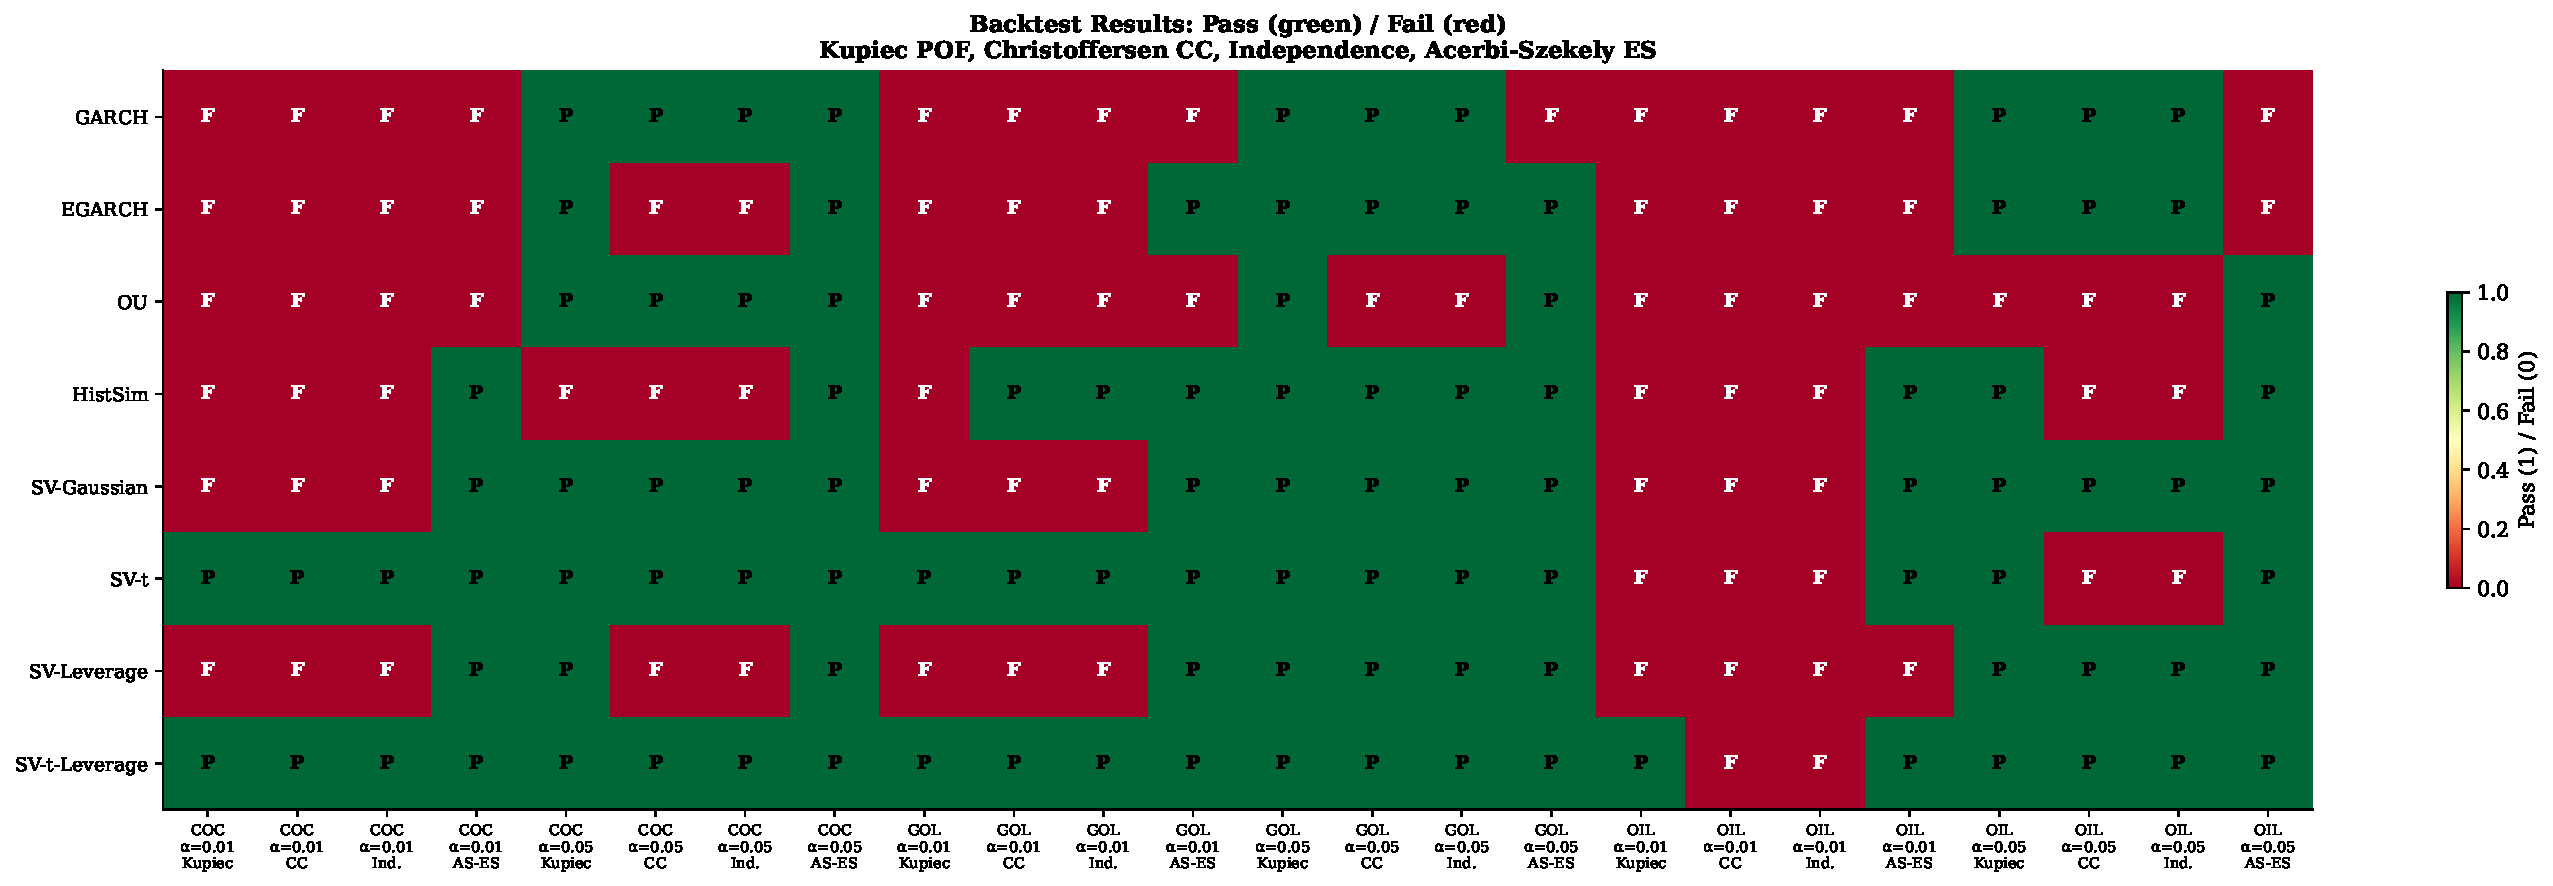
\includegraphics[width=\textwidth]{figs/fig4_backtest_heatmap.pdf}
\caption{Pass (green) / fail (red) outcome for every backtest reported in Table~\ref{tab:backtest_main}, across all eight models, three commodities, two confidence levels, and three test statistics. The visual density of green cells for cocoa and gold versus the persistent red band for oil at 99\% VaR (Kup.\ column) makes the paper's central differentiated finding immediately legible: adequacy is achievable for cocoa and gold but not, at this confidence level, for oil.}
\label{fig:heatmap}
\end{figure}

\subsection{A Cross-Commodity Diagnostic: Ornstein--Uhlenbeck Convergence}
\label{sec:results_ou}

One further result deserves attention on its own terms, separate from the VaR backtests above, because it was a diagnostic built directly into the evaluation framework in Section~\ref{sec:ou} rather than an incidental observation. For each rolling window, we recorded whether the OU model's mean-reversion parameter $\hat{\kappa}_i$ exceeded our pre-specified threshold of $0.01$; where it did not, we treated the window as non-convergent rather than force a spurious estimate. The resulting non-convergence rate differs meaningfully across the three commodities: 4.3\% of windows for cocoa, 10.7\% for gold, and 5.1\% for oil.

Gold's rate is more than double that of either cocoa or oil. This is precisely the pattern one would expect on the strength of \citet{bessembinderetal1995}, whose classical analysis of futures term structures found mean reversion to be economically large for agricultural commodities and crude oil, but substantially weaker for precious metals. We had, on the strength of that paper, anticipated this asymmetry before running the estimation, and it is gratifying, though not something we take as more than suggestive given the different methodologies involved, that a diagnostic built into our own rolling-window procedure for an entirely different purpose --- flagging non-convergent OU windows so they could be honestly excluded from the violation count --- independently reproduces a pattern first documented in the finance literature three decades ago.

\subsection{Robustness Checks: Status}
\label{sec:robustness_status}

Section~\ref{sec:evaluation} pre-committed this study to six robustness checks: variation in the rolling-window length ($W \in \{750, 1{,}000, 1{,}250\}$), re-estimation of the core cocoa results with the three flagged 2024 rollover-illiquidity dates excluded, re-estimation of cocoa using the ICCO composite price series in place of Yahoo Finance's CC=F, re-estimation of oil using the Yahoo WTI futures series in place of the primary Brent spot series, a prior-sensitivity check under a flatter specification for $\phi_i$ and $\sigma_{\eta,i}$, and a GARCH order check against GARCH$(1,2)$ and GARCH$(2,1)$ specifications.

None of these six checks had been executed at the time of writing this section. We state this without qualification, because presenting the primary results as though they were robustness-confirmed, when they are not yet, would be a more serious error than the gap itself. The results reported in Sections~\ref{sec:results_cocoa}--\ref{sec:results_ou} rest entirely on the single primary specification: $W=1{,}000$, the primary Brent and Yahoo CC=F price series, the priors specified in Table~\ref{tab:priors}, and GARCH$(1,1)$/EGARCH$(1,1)$ justified a priori rather than confirmed by order search on this data. Completing the six pre-committed checks is the immediate next step following this study, not a parallel track that happened not to make it into this document, and we would regard any of the headline findings above --- particularly the cocoa leverage result and the oil non-result --- as provisional rather than fully established until at least the window-length and alternative-price-source checks have been completed.

\subsection{From Results to Discussion}

Taken together, these results do not resolve into a single winning model. They resolve into something we think is more useful: a differentiated, commodity-specific account of where a richer volatility specification earns its complexity and where it does not. Student-$t$ innovations are necessary and, for gold specifically, sufficient; the leverage channel adds real value for cocoa in a way it does not for gold; and oil resists every specification we estimate, benchmark or primary alike, at the 99\% confidence level regulatory practice treats as the operative standard. The Discussion that follows takes up what this pattern means in practice --- for how a Ghanaian institution such as COCOBOD might reasonably interpret a cocoa risk model that finally clears the bar existing benchmarks do not, and for how a risk manager exposed to oil should treat a result in which the best available model, however carefully specified, still fails the very test regulatory convention regards as decisive.

\section{Discussion}
\label{sec:discussion}

What follows is not a second pass through the numbers reported in Section~\ref{sec:results}. It is an attempt to work out what those numbers actually mean --- for a Ghanaian institution managing real commodity exposure, for how this study sits against the literature it builds on, and for what we still do not know, some of it because we have not yet had time to check, some of it because the data itself has not given up an answer. We take the last of these as seriously as the first two.

\subsection{Why a Single Winning Model Was Never the Right Expectation}

It would have been convenient, and we do not think it would have been correct, if one specification had swept every backtest for every commodity. The stylised facts established in Section~\ref{sec:stylised} describe three genuinely different empirical situations, not three noisy draws from one underlying truth. Cocoa carries a detectable, if modest, asymmetric volatility response; gold does not, or at least not one strong enough to reward modelling it; oil's return distribution is shaped by a small number of episodes so extreme that its excess kurtosis exceeds gold's by more than a factor of twelve. A single model built to be best on average across these three situations would necessarily be worse than the commodity-specific answer this study arrives at instead --- adequate for gold on its own terms, adequate for cocoa only once leverage is modelled explicitly, and, for oil, not adequate at all at the confidence level regulatory convention treats as decisive. We think this differentiated outcome is the more useful one to report, even though it resists the tidier headline a single dominant model would have offered.

There is a point here that goes beyond methodology, and we raised it once already, in the ethics discussion of Section~\ref{sec:ethics}, in a way we want to return to substantively rather than leave as a passing remark. Among the models that fit cocoa best in this study --- SV-$t$-Leverage, the specification producing the smallest deviation from nominal coverage of any model estimated anywhere in this paper --- the commodity fitted happens to be the one among our three that is not, for Ghana, simply a financial instrument. A large share of Ghanaian smallholder farmers depend on cocoa income directly, and the volatility this paper models has a bearing, however indirect, on COCOBOD's hedging decisions and on the country's export earnings. We do not think this coincidence carries any deep methodological significance --- the leverage effect is present in cocoa's own return series for reasons of market structure and supply shock, not because the commodity matters more to Ghana than gold or oil do. But we also do not think it is honest to notice this outcome and say nothing about it. A model that works particularly well for the commodity with the most immediate human stakes in this study is, we think, worth building on rather than treating as an incidental result to file alongside the others.

\subsection{Practical Implications for Risk Management}

\subsubsection{Cocoa}

A model that reliably clears the 99\% VaR bar where GARCH, EGARCH, the Ornstein--Uhlenbeck benchmark, and Historical Simulation all fail is not, on its own, a policy prescription. We want to be modest about what it does offer. An institution with cocoa exposure --- COCOBOD itself, a Ghanaian bank financing cocoa trade, or a stabilisation fund sized against expected price swings --- currently has no adequately calibrated benchmark among the standard tools this study tested. SV-$t$-Leverage's clean sweep suggests such an institution could, in principle, size a risk buffer against a 99\% daily VaR figure with more confidence than any of the four benchmark models would currently support. This is a genuinely useful, if narrow, practical contribution: better-calibrated inputs to a hedging or reserve-sizing decision, not a claim that cocoa price risk has become predictable or that a stabilisation fund's overall adequacy reduces to getting one daily statistic right.

\subsubsection{Gold}

The gold result needs less unpacking, precisely because it is cleaner: SV-$t$ passes all six backtests, and the story is close to the textbook case for why heavy-tailed innovations matter without a leverage complication layered on top. For a Ghanaian institution with gold exposure --- and Ghana is a significant gold producer, with real fiscal and export-revenue stakes in the commodity --- this is good news as far as it goes. But we want to flag a distinction that matters for how directly this transfers into practice: the series we model throughout this study is a global, internationally traded futures price, not a Ghana-specific producer price or the price actually realised by a domestic mining operation after local costs, royalties, and contractual arrangements are accounted for. The backtest evidence supports treating SV-$t$ as an adequate model of \emph{global gold price risk}. Whether that risk transmits one-for-one into the risk faced by a specific Ghanaian producer or exporter is a separate empirical question this study does not answer.

\subsubsection{Oil}

This is the hardest and, we think, the most practically important implication in the paper, precisely because the honest answer is not reassuring. If no model we estimate --- including the richest specification available to us --- reliably captures oil's 99\% tail risk, what should an oil-import-exposed Ghanaian institution or policymaker actually do with that finding? We do not think the right conclusion is to abandon quantitative oil risk modelling; a model that fails a strict backtest is still informative, and SV-$t$-Leverage's 59 violations against 48 expected is a meaningfully better forecast than GARCH's 80 or EGARCH's 86, even though none of them clears the bar. The conclusion we do draw is that a single VaR number for oil should be treated with real caution, not taken as a settled, sufficient description of tail risk. Two practical responses follow directly from our own results, rather than from generic risk-management advice. First, the crisis-period shading in Figure~\ref{fig:returns_overview} --- built around the GFC, COVID-19, the 2024 cocoa crisis, and the 2026 Middle East-driven oil shock --- gestures toward exactly the kind of named-scenario stress-testing that should sit alongside, not instead of, any point-estimate VaR figure for oil specifically; a model that cannot pass a statistical backtest built around ordinary historical variation can still be usefully paired with an explicit scenario asking, concretely, what a repeat of April 2020 or February 2026 would do to a given exposure. Second, an institution relying on any of the models in this study for oil should hold larger capital or liquidity buffers than a technically adequate-looking VaR figure would, on its own, suggest is necessary --- precisely because we have shown, directly and repeatedly across eight different specifications, that adequate-looking is not the same as adequate.

\subsection{Position Relative to Existing Literature}

The closest methodological precedent to this study is \citet{tweneboah2025}\footnote{We have confirmed this paper studies the Ghana Stock Exchange Composite Index from 2011--2022 using four Bayesian stochastic volatility variants --- linear regressors, Student-$t$ errors, leverage effects, and a combined Student-$t$-with-leverage hybrid --- published in \textit{Risks} (MDPI), with the Student-$t$ variant identified as most effective by RMSE. We have not independently confirmed the exact volume, issue, and article number for this citation and flag this rather than guess at it.}, which applies Bayesian latent stochastic volatility, including a leverage-effect specification, to Ghanaian equity data. What we add beyond that precedent is threefold: an extension from a single equity index to three commodities with materially different volatility characteristics; a genuine cross-commodity comparison rather than a single-series application; and an explicit, pre-registered VaR and Expected Shortfall backtesting framework, using three complementary statistics, rather than in-sample fit criteria alone. We regard \citet{tweneboah2025} as evidence that the methodological toolkit we use is already established for Ghanaian financial data; our contribution is to show where, and where not, it holds up once evaluated against genuinely out-of-sample tail-risk criteria for commodities specifically.

A separate strand of Ghana-specific literature examines dependence and comovement between commodity prices and Ghanaian macroeconomic variables directly: \citet{boateng2022} on the interconnectedness of cocoa, Brent crude, and gold with Ghana's real sector; \citet{yeboah2025} on asymmetric dependence between cocoa, oil, gold, and Ghanaian macroeconomic variables; and \citet{barson2023} on exchange-rate-conditioned commodity comovement using wavelet methods. These studies and the present one are complementary rather than competing: they ask whether and how commodity prices move together with Ghana's exchange rate, inflation, and real economic activity; we ask whether a given commodity's own tail risk can be adequately modelled at all, independent of any macroeconomic conditioning variable. A natural extension of this study, which we return to below, would condition the volatility models estimated here on exactly the kind of exchange-rate and macroeconomic variables this literature has already shown to matter.

We want to revisit, one further time and in a different register, the contrast between \citet{chenzerillibaum2019} and \citet{kuang2022} on oil VaR modelling. In Section~\ref{sec:results_oil} we treated this as a piece of corroborating evidence for our own finding. Here we want to draw out what it implies beyond this paper. If two published, peer-reviewed studies using broadly similar Bayesian stochastic volatility machinery reach opposite conclusions about whether fat-tailed innovations are necessary for oil risk, and the most plausible explanation is simply which crises their respective samples happen to include, that is a genuinely uncomfortable fact for the field, not only for this study. It suggests that published claims about model adequacy for oil tail risk should be read with an eye to the sample window before being generalised, and that a specification's apparent success may say as much about which historical episodes it was tested against as about the specification itself. We do not think this undermines the value of backtesting; if anything, it is an argument for exactly the kind of pre-registered, multi-decade, crisis-inclusive evaluation this study attempts.

\subsection{Limitations}

Section~\ref{sec:robustness_status} already reported, without qualification, that none of the six pre-committed robustness checks had been completed at the time of writing. We do not want to leave that as a bare admission; it matters, differently, for different results in this paper. If the cocoa leverage finding turned out to depend heavily on excluding the three flagged 2024 rollover-illiquidity dates, that would meaningfully soften what is currently the paper's cleanest result --- we would want to know whether SV-$t$-Leverage's clean sweep survives with those dates retained, and we do not yet know the answer. If the ICCO-price-source robustness check moved the cocoa result at all, that would implicate something we already flagged as unresolved in Section~\ref{sec:data}: the residual, roughly two-percent gap between the Yahoo CC=F series and ICCO's New York leg that survives even after accounting for contract-month blending. We do not currently know whether that unexplained gap is large enough to matter for a VaR backtest specifically, as opposed to a simple price-level comparison, and this is precisely the kind of question the pending robustness check was designed to answer.

The rolling-window SV estimation itself carries a computational compromise we described plainly in Section~\ref{sec:sv}: full re-estimation every 42 trading days rather than at every step, using a single MCMC chain in the rolling context against four chains in full-sample estimation. We do not think this invalidates the results, since the same compromise applies uniformly across all four SV variants and should not, on its own, favour one over another. But it could plausibly understate how much the SV models' posterior uncertainty grows between refits, particularly around the crisis episodes --- 2008, 2020, 2024, 2026 --- where volatility regimes shift fastest and where a stale posterior is most likely to be wrong. We flag this as a real, not merely formal, limitation.

Our reliance on a third-party Kaggle repository for the pre-2024 portion of the extended ICCO cocoa series is a further limitation worth restating here rather than only in the Data section. We validated that repository against an independently obtained official ICCO export, but only for the window where both were available --- October 2024 through August 2025. The earlier years, on which the repository's real usefulness depends, were validated only by inference from that later agreement, not by direct comparison against ground truth we do not have.

The 2025 persistence of an elevated WTI futures-spot basis, noted in Section~\ref{sec:data} against the documented late-2024 shift toward contango, remains genuinely unexplained. We do not use the WTI series as our primary oil measure, so this does not bear directly on the headline results, but it is an open question in this paper's own data-validation work that we have not resolved and do not want to present as settled.

Finally, we think it is worth stating plainly, without excessive self-deprecation, that this is a single-author study conducted without institutional computational infrastructure or a research team. That constraint shaped real, specific choices --- the 1,000-day window length, the 42-day refit interval, the decision to defer Heston and SABR entirely rather than attempt an under-resourced version of either --- in ways a better-funded project might not have needed to make. We do not think those choices were unreasonable given the constraint; we do think a reader should know the constraint was real, not merely mentioned as a formality.

\subsection{Contribution}

What this study contributes is not a universally superior volatility model. It is a rigorously backtested, commodity-differentiated account of where Bayesian latent stochastic volatility earns its additional complexity, for three commodities of direct relevance to a West African economy, evaluated against a framework of tests and thresholds committed to in writing before any model saw the data it would eventually be judged against. That last point is not incidental to the contribution; it is a substantial part of it. A comparison assembled after seeing which model looked best would be a weaker piece of evidence than the one this paper reports, regardless of whether the headline numbers came out the same.

\subsection{Future Work}

The immediate next step is not a new direction but the six checks already pre-committed and not yet run: window-length variation, the cocoa date exclusion, the alternative cocoa and oil price sources, prior sensitivity, and the GARCH order check. We regard the cocoa and oil headline findings in this paper as provisional, not final, until at least the price-source and window-length checks are complete.

Beyond that, the oil non-result raises a specific question we did not have standing to ask before seeing it: is a continuous-time jump-diffusion extension, closer in spirit to \citet{trolleschwartz2009}'s treatment of unspanned stochastic volatility in commodity derivatives, a more promising direction for oil specifically than continuing to search within the discrete-time SV family we have exhausted here? We do not think our results answer this question, but they narrow it usefully: a smooth, heavy-tailed but still continuous innovation distribution has now failed four separate times for oil in this study alone, which is at least suggestive that the problem is one of functional form --- discrete jumps versus smooth tails --- rather than simply insufficiently heavy tails.

A further, more Ghana-specific extension would replace the international CC=F cocoa series used throughout this study with a genuine domestic producer-price series, closer to what a Ghanaian cocoa farmer or COCOBOD itself actually faces after forward-sales arrangements and fixed producer pricing are accounted for. Such an extension would let this study's tail-risk framework speak directly to the price farmers realise, rather than only to the international benchmark from which that price is ultimately derived.

\subsection{From Discussion to Conclusion}

We have tried, in this section, to take the differentiated pattern established in Section~\ref{sec:results} seriously on its own terms --- as three separate answers to three separate empirical situations, not as an untidy result to be smoothed into a single verdict. What remains is to state, briefly and without repeating the reasoning above, what this study has actually established and where it leaves the questions it opened.

\section{Conclusion}
\label{sec:conclusion}

We set out to answer a specific question: whether Bayesian latent stochastic volatility models provide adequately calibrated tail-risk forecasts for cocoa, gold, and crude oil, three commodities of direct and distinct significance to Ghana and West Africa, and whether the answer is the same across all three. It is not. Student-$t$ innovations resolve gold's tail-risk calibration problem cleanly, with a perfect backtest pass rate across every test we ran. Cocoa needed more: only the combination of Student-$t$ innovations and an exactly derived leverage channel achieved the same result, a finding that agrees with an independent, differently modelled precedent in the agricultural commodity literature. Oil resisted every specification we estimated, benchmark and primary alike, at the 99\% confidence level regulatory practice treats as the operating standard --- not because the modelling effort was inadequate, but because the underlying return distribution, shaped by a small number of extraordinary crisis episodes, may exceed what any single smooth parametric family can be asked to represent.

Every one of these findings rests on an evaluation framework fixed in writing before a single model touched the data it would eventually be judged against: the rolling window length, the backtest statistics, the pass-count ranking criterion, and the robustness checks were all committed to in Section~\ref{sec:methodology}, not assembled after the fact to fit whatever result came out best. We regard this discipline as inseparable from the paper's contribution rather than a procedural footnote to it.

The work that remains is concrete rather than open-ended: the six pre-committed robustness checks reported as outstanding in Section~\ref{sec:robustness_status}, a Ghana-specific producer-price extension for cocoa, and a genuine test of whether a jump-diffusion alternative succeeds where four different smooth-tailed specifications did not for oil. We have tried, throughout this paper, to report what we found rather than what would have made the tidiest story, and we close it in the same spirit: this is a differentiated, partial, and honestly limited answer to a real question facing a real economy, not a final one.

\bibliographystyle{elsarticle-harv}
\begin{thebibliography}{99}

\bibitem[Acerbi and Sz\'ekely(2014)]{acerbiszekely2014}
Acerbi, C., \& Sz\'ekely, B. (2014). Back-testing expected shortfall. \textit{Risk Magazine}, December, 76--81.

\bibitem[Barson et al.(2023)]{barson2023}
Barson, Z., Owusu Junior, P., \& Adam, A. M. (2023). Comovement between commodity returns in Ghana: The role of exchange rates. \textit{Journal of Economic Structures}, 12, Article 17. https://doi.org/10.1186/s40008-023-00312-z

\bibitem[Bessembinder et al.(1995)]{bessembinderetal1995}
Bessembinder, H., Coughenour, J. F., Seguin, P. J., \& Smoller, M. M. (1995). Mean reversion in equilibrium asset prices: Evidence from the futures term structure. \textit{The Journal of Finance}, 50(1), 361--375. https://doi.org/10.1111/j.1540-6261.1995.tb05178.x

\bibitem[Boateng et al.(2022)]{boateng2022}
Boateng, E., Asafo-Adjei, E., Addison, A., Quaicoe, S., Yusuf, M. A., Abeka, M. J., \& Adam, A. M. (2022). Interconnectedness among commodities, the real sector of Ghana and external shocks. \textit{Resources Policy}, 75, Article 102511. https://doi.org/10.1016/j.resourpol.2021.102511

\bibitem[Bollerslev(1986)]{bollerslev1986}
Bollerslev, T. (1986). Generalized autoregressive conditional heteroskedasticity. \textit{Journal of Econometrics}, 31(3), 307--327. https://doi.org/10.1016/0304-4076(86)90063-1

\bibitem[Chen et al.(2019)]{chenzerillibaum2019}
Chen, L., Zerilli, P., \& Baum, C. F. (2019). Leverage effects and stochastic volatility in spot oil returns: A Bayesian approach with VaR and CVaR applications. \textit{Energy Economics}, 79, 111--129. https://doi.org/10.1016/j.eneco.2018.03.032

\bibitem[Christoffersen(1998)]{christoffersen1998}
Christoffersen, P. F. (1998). Evaluating interval forecasts. \textit{International Economic Review}, 39(4), 841--862.

\bibitem[Hansen and Lunde(2005)]{hansenlunde2005}
Hansen, P. R., \& Lunde, A. (2005). A forecast comparison of volatility models: Does anything beat a GARCH(1,1)? \textit{Journal of Applied Econometrics}, 20(7), 873--889. https://doi.org/10.1002/jae.800

\bibitem[Hosszejni and Kastner(2019)]{hosszejnikastner2019}
Hosszejni, D., \& Kastner, G. (2019). Approaches toward the Bayesian estimation of the stochastic volatility model with leverage. In R. Argiento, D. Durante, \& S. Wade (Eds.), \textit{Bayesian Statistics and New Generations} (Springer Proceedings in Mathematics \& Statistics, Vol. 296, pp. 75--83). Springer. https://doi.org/10.1007/978-3-030-30611-3\_8

\bibitem[Jacquier et al.(1994)]{jacquierpolsonrossi1994}
Jacquier, E., Polson, N. G., \& Rossi, P. E. (1994). Bayesian analysis of stochastic volatility models. \textit{Journal of Business \& Economic Statistics}, 12(4), 371--389.

\bibitem[Jacquier et al.(2004)]{jacquierpolsonrossi2004}
Jacquier, E., Polson, N. G., \& Rossi, P. E. (2004). Bayesian analysis of stochastic volatility models with fat-tails and correlated errors. \textit{Journal of Econometrics}, 122(1), 185--212. https://doi.org/10.1016/j.jeconom.2003.09.001

\bibitem[Kastner and Fr\"uhwirth-Schnatter(2014)]{kastnerfruhwirthschnatter2014}
Kastner, G., \& Fr\"uhwirth-Schnatter, S. (2014). Ancillarity-sufficiency interweaving strategy (ASIS) for boosting MCMC estimation of stochastic volatility models. \textit{Computational Statistics \& Data Analysis}, 76, 408--423. https://doi.org/10.1016/j.csda.2013.01.002

\bibitem[Kim et al.(1998)]{kimshephardchib1998}
Kim, S., Shephard, N., \& Chib, S. (1998). Stochastic volatility: Likelihood inference and comparison with ARCH models. \textit{The Review of Economic Studies}, 65(3), 361--393. https://doi.org/10.1111/1467-937X.00050

\bibitem[Kuang(2022)]{kuang2022}
Kuang, W. (2022). Oil tail-risk forecasts: From financial crisis to COVID-19. \textit{Risk Management}, 24(4), 420--460.

\bibitem[Kupiec(1995)]{kupiec1995}
Kupiec, P. H. (1995). Techniques for verifying the accuracy of risk measurement models. \textit{The Journal of Derivatives}, 3(2), 73--84. https://doi.org/10.3905/jod.1995.407942

\bibitem[Nelson(1991)]{nelson1991}
Nelson, D. B. (1991). Conditional heteroskedasticity in asset returns: A new approach. \textit{Econometrica}, 59(2), 347--370.

\bibitem[Roux(2018)]{roux2018}
Roux, C. L. (2018). Volatility modelling of agricultural commodities: Application of selected GARCH models. In N. Tsounis \& A. Vlachvei (Eds.), \textit{Advances in Panel Data Analysis in Applied Economic Research} (Springer Proceedings in Business and Economics, pp. 343--356). Springer.

\bibitem[Trolle and Schwartz(2009)]{trolleschwartz2009}
Trolle, A. B., \& Schwartz, E. S. (2009). Unspanned stochastic volatility and the pricing of commodity derivatives. \textit{The Review of Financial Studies}, 22(11), 4423--4461. https://doi.org/10.1093/rfs/hhp036

\bibitem[Tweneboah et al.(2025)]{tweneboah2025}
Tweneboah, G., Ohene-Obeng, K. A., \& Mariani, M. C. (2025). Stochastic volatility modelling of the Ghana Stock Exchange Composite Index using Bayesian methods. \textit{Risks} (MDPI). \emph{[Exact volume, issue, and article number not independently confirmed; study subject matter --- GSE-CI, 2011--2022, four Bayesian SV variants with Student-$t$ identified as most effective --- has been confirmed.]}

\bibitem[Yeboah et al.(2025)]{yeboah2025}
Yeboah, S. D., Fumey, M. P., Winful, S. A., Otoo, I. C., \& Owusu Junior, P. (2025). Asymmetric dependence between commodity prices and selected macroeconomic variables in Ghana. \textit{Scientific African}, 28, Article e02739. https://doi.org/10.1016/j.sciaf.2025.e02739

\end{thebibliography}
\end{document}
